\documentclass[a4paper, oneside]{discothesis}

\usepackage[utf8]{inputenc}
\usepackage[T1]{fontenc}
\usepackage{graphicx}
\usepackage{float}
\usepackage{cprotect}
\usepackage{listings}
\usepackage{xcolor}
\usepackage{dirtree}
\usepackage{mathtools}
\usepackage{comment}
\usepackage[labelfont=bf,font=small,skip=5pt]{caption}
\usepackage[outdir=./figures/]{epstopdf}
\usepackage{titlesec}

\usepackage[utf8]{inputenc}
\usepackage[T1]{fontenc}
\usepackage{graphicx}
\usepackage{float}
\usepackage{cprotect}
\usepackage{listings}
\usepackage{xcolor}
\usepackage{dirtree}
\usepackage[labelfont=bf,font=small,skip=5pt]{caption}

\setcounter{secnumdepth}{3}
\usepackage{hyperref}


\definecolor{codegreen}{rgb}{0,0.6,0}
\definecolor{codegray}{rgb}{0.5,0.5,0.5}
\definecolor{codepurple}{rgb}{0.58,0,0.82}
\definecolor{backcolour}{rgb}{0.95,0.95,0.92}


\lstdefinestyle{mystyle}{
	backgroundcolor=\color{backcolour},   
	commentstyle=\color{codegreen},
	keywordstyle=\color{magenta},
	numberstyle=\tiny\color{codegray},
	stringstyle=\color{codepurple},
	basicstyle=\ttfamily\footnotesize,
	breakatwhitespace=false,         
	breaklines=true,                 
	captionpos=b,                    
	keepspaces=true,                 
	numbers=left,                    
	numbersep=5pt,                  
	showspaces=false,                
	showstringspaces=false,
	showtabs=false,                  
	tabsize=2
}
\lstset{style=mystyle}


%%%%%%%%%%%%%%%%%%%%%%%%%%%%%%%%%%%%%%%%%%%%%%%%%%%%%%%%%%%%%%%%%%%%%%%%%%%%%%%%%%%%%%%%%%%%%%%%%
% DOCUMENT METADATA

\thesistype{Master's thesis} % Master's thesis, Bachelor's thesis, Semester thesis, Group Project
\title{On fast simulations of cardiac function}

\author{Diego Renner}
\email{drenner@student.ethz.ch}

\institute{Dep. of Mathematics \\[2pt]
ETH Zürich}

% Optionally, you can put in your own logo here

\supervisors{Prof. Dr. Siddhartha Mishra}

% Optionally, keywords and categories of the work can be shown (on the Abstract page)
%\keywords{Keywords go here.}
%\categories{ACM categories go here.}

\date{\today}

%%%%%%%%%%%%%%%%%%%%%%%%%%%%%%%%%%%%%%%%%%%%%%%%%%%%%%%%%%%%%%%%%%%%%%%%%%%%%%%%%%%%%%%%%%%%%%%%%

\begin{document}

\frontmatter % do not remove this line
\maketitle
\cleardoublepage

\begin{acknowledgements}
	
\end{acknowledgements}


\begin{abstract}
	
\end{abstract}

\tableofcontents

\mainmatter % do not remove this line

\chapter{Introduction}

By taking into account the characteristics of an individual patient and customizing the treatment this patient receives according to which characteristics-dependent sub-population this patient falls into, personalized medicine aims to improve upon results a more generalized approach would achieve \cite{ashley2016towards,national2011toward,giardino2017role}.
To succeed in the personalization of a treatment, a disease specific number of quantities (biomarkers) need to be determined \cite{burke1998integrating}.
These biomarkers can have a varying degree of correlation with a diseases existence, progression, and outcome.
For instance local vascular pressure is highly correlated with hypertension.
While there are methods to estimate this quantity from ultrasound or Magnetic Resonance Imaging \cite{markl20124d}, these methods tend not to be accurate enough for standard clinical practice \cite{everett2012beyond}.
On the other hand more invasive techniques might not offer the proper risk to reward ratio.
For example, to diagnose hypertensive pregnancy disorder it would be very risky to perform the measurement of the absolute vascular pressure in-vivo on a pregnant subject \cite{kett2002adverse}.
Therefore in order to determine the biomarkers that are hard to capture in a clinical setting computational methods are often applied.

Such computational models aim to simulate a patients individual physiology in order to reveal aforementioned "hidden" biomarkers.
The prerequisite for this to work is that biomarkers can be simulated that are strongly show strong correlations with a disease.
For example being able to determine the genetic predisposition of a patient with respect to a certain disease would be a very strong indicator of the outcome od said disease.
However this cannot be attempted with such methods.
On the otherhand for instance the local vascular pressure, or the resistance within a cardiovascular network are good indicators that can in fact be simulated due to the underlying physics being well understood.
However the simulations depend heavily on a high number of personalized parameters, leading to a similar problem as described initially: needing to access difficult to measurable or unobtainable data for a specific patient.
An attempt to avoid the problem of having to know these values is using population averaged values.
This however defeats the purpose of personalized medicine.
What has therefore become the method of choice to address the issue of personalized medicine using computational models is to build simulators that output the values of some desired biomarkers and to then try and solve the inverse problem of fitting the parameters of the simulator to a specific patient.

There are two main ways of achieving the goal of calibrating a simulation for an individual
\begin{enumerate}
	\item A "classical" approach, where the inverse problem is solved using Markov-Chain-Monte-Carlo \cite{melis2017gaussian}, or Kalman filters \cite{manganotti2022modeling}.
	\item A Deep-Learning approach where the calibration is avoided all together in favor of learning the model from data. \cite{kissas2020machine,arzani2022machine}
\end{enumerate}
The reason Deep-Learning techniques were attempted is due to the fact that the "classical" approaches are very inefficient.
This is because the derivatives are often hard to determine for the attempted simulations so the algorithms of choice for solving the inverse problem are gradient-free. 
Moreover due to the models being very sensitive to it's parameters and there being ambiguous solutions \cite{nolte2022inverse,quick2001infinite} these gradient-free algorithms have to be run at very small step sizes. \cite{taylor2009patient,tuccio2022parameter,marsden2014optimization,mineroff2019optimization,bozkurt2022patient}
The ability to easily take gradients of one of these models with respect to it's parameters would greatly improve the process of personalizing them without loosing the interpretability as would be the case when using a Deep-Learning algorithm.

Due to the complexity of the cardiovascular system and the significance of cardiovascular disease globally the mathematical and numerical modelling of haemodynamics has gained a lot of traction over recent years.
Two of the main factors for this complexity are the multi-scale and multi-physics nature of the cardiovascular system that arises from vessels of strongly varying sizes and not much data being available for certain parts of these models to go off of \cite{quarteroni2016geometric}.

The motivation for researching cardiovascular disease stems from it being the most prevalent cause of death.
Worldwide it leads 17.3 million deaths per year as of 2015.
This number is projected to increase by the year 2030 to more than 23.6 million. \cite{update2015heart}
In Europe cardiovascular disease was responsible for close to one third (32.7\%) of all deaths in the year 2020 \cite{Coelho2020}.
In order to tackle the complexity of the meaningful task of modelling cardiovascular systems numerical modelling has become prevalent \cite{formaggia2009multiscale,quarteroni2016geometric,black2020p14,el2018investigating,qureshi2014numerical,reichold2009vascular}.
The general issue described up until now with regards to the difficulty of personalizing treatments is also relevant when considering the cardiovascular system.

Therefore the goal of this work is to provide a fast, differentiable cardiovascular simulation.
This is a step towards enabling efficient and interpretable model calibration to be applied in personalised medicine.
In order to be differentiable the haemodynamics solver written in the course of this thesis was written using the JAX library.
On top of differentiability JAX also offers device agnostic execution.
JAX optimizes the executed code to take advantage of parallelization and other advantages of modern hardware regardless of if it's being executed on a CPU, GPU or TPU.
The optimization for GPU execution is especially useful since it allows for data paralellization, i.e. batch executions of the code on a single device.
This means multiple models for different patients could be optimized simultaneously on a single GPU.
Next to the advantages brought about by the implementation in JAX, the implementation of the code in Python makes the solver accessible for future work.
We also provide the written code as is in an open-source manner hoping to aid progress in the field overall.

For this thesis we chose a coupled 0D-1D model where the 0D part is used to compute boundary conditions for certain outlets of the 1D cardiovascular network.
While failing to capture complex flow patterns and wall shear stress as opposed to a 3D model the 1D model can still simulate pulse wave transmission and systemic wave reflection effects.
Clearly 1D models also offer a big advantage in execution time as opposed to 3D models. \cite{shi2011review,pfaller2020using,arzani2022machine} 
In the next section we will provide a basic understanding of the cardiovascular system which will serve as a base for describing the cardiovascular simulation throughout this work.




% 1) Introduction
% why cardiovascular simulation important
% description of the current ways to simulate
% description of the problems/limitations of these methods
% how our approach works
% and _why_ it solves issues of previous methods
% list specific contributions:
    % a 1D solver which is
    % - written for GPU on JAX
    % - highly scalable (multi-GPU / device agnostic)
    % - differentiable
    % - open source
    % - easy to understand (written in python)
% future work / impact it will have in the future
    % path towards complex, real-world simulation
    % digital twin, data assimilation, etc ..

% 2) Cardiovascular system
% why cardiovascular simulation important

% 3) 1D Model
% mathematical model

% 4) Existing numerical models
% description of the current ways to simulate
% description of the problems/limitations of these methods

% 5) Our implementation
% how our approach works
% and _why_ it solves issues of previous methods
% nice overview diagram showing workflow

% 6) Results & benchmarks
% timing tests / accuracy compared to Julia model
% GPU vs CPU time
% scaling tests:
    % computational time vs number of vessels
    % vmap multiple simulations
% time to compute gradients / linear approximation of function

% 7) Discussion
% future work / impact it will have in the future
    % multi-GPU
    % sensitivity tests
    % open-sourcing
% maybe including proof-of-principle inverse test

% 8) Conclusions 
% (repeat contribution / impact)

\chapter{Cardiovascular System}
This section serves as an overview of the cardiovascular system with a focus on the arteries of the systemic circulation. 
Section \ref{mbb} will describe the main building blocks of the cardiovascular system and their relation, section \ref{aw} will give the characteristics of the arterial walls, and section \ref{b} the characteristics of blood.
\section{Main Building Blocks} \label{mbb}
The cardiovascular system contains two major circulatory systems.
These are the systemic and the pulmonary circulation. 
Both are fed with blood pumped from the heart.
Through the systemic circulation organs are supplied with oxygen-rich blood which is then transported back to the heart where it then enters the pulmonary circulation.
Through the pulmonary circulation the oxygen-poor blood is sent to the lungs where it is replenished with oxygen and then returned to the heart to reenter the systemic circulation.
Vessels carrying the blood away from the heart are referred to as arteries and the ones carrying the blood to the heart are referred to as veins.
In both the systemic and the pulmonary circulation the oxygen exchange (from blood to organs or from lungs to blood respectively) take place within so called capillary vessels.
Capillaries are very small vessels that connect arteries to veins.
From here on out our main focus will be on on the arteries of the systemic circulation. 
In the next two subsections we will describe the main characteristics of the arterial walls and the blood flowing within.

\section{Arterial Wall} \label{aw}
An arterial wall consists of three layers or tunicae: an inner, middle, and outer layer also referred to as intima, media, and adventita respectively.
The tunica intima lines the inside of the artery. It is made up of a single layer of endothelial cells encased in a thin layer of elastin and collagen fibres (connective tissue). 
On the outside of the artery the tunica adventita is made up of connective tissue as well which attaches the artery to surrounding connective tissue.
In-between these two layers lies the thickest layer, the tunica media, which consists of elastic fibres and muscle cells. 
The tunica media is responsible for the elasticity of the artery.
Arteries close to the heart have a tunica media that is mainly made up of elastic fibres and are referred to as elastic arteries while the tunica media of arteries farther away from the heart and of small arteries consist predominantly of muscle cells and are called muscular arteries.
The elastic arteries also have a higher compliance.
This means that that they are able to distended and increase their volume as a response to pressure applied to the inside of the arterial wall.
Hence elastic arteries deform more under the than the muscular arteries that are stiffer when blood is pumped into them by the heart.
At the same time usually the elastic arteries are larger than the muscular arteries and the size of arteries generally descends as the distance to the heart increases.
The compliance of the larger elastic arteries is responsible for transforming the pulsatile flow at the heart into a constant flow at the capillaries.
The pulse-like pressure change coming from the heart leads to the elastic arteries close to the heart expanding.
Until the next pulse arrives these vessels will contract slowly, pushing the blood at a constant rate into the arteries farther away from the heart and finally into the capillaries.
This mechanism is called the Windkessel effect.
It is named after the inner workings of waterpumps used by early fire brigades.
In these devices water would be pumped by hand from the reservoir causing pressure pulses.
This would push water into an air chamber.
Here the air would get compressed which is analogous to the deforming of the artery.
The natural decompressing of the air would then push the water out through the hose in a steady manner, just like the contracting of the artery would push out the blood.
The Windkessel effect is often applied in vascular simulations to apply outlet boundary conditions.
We will describe how this is done more closely in \autoref{sssec:outl}.
For further reference in the following chapters we will also introduce some notation.
We call the radius of an artery in it's undeformed state the lumen radius $r_0$ and refer to the reference vessel wall thickness by $h_0$ from here on out.
Furthermore we denote the reference cross-section by $A_0 = \pi r_0^2$.

\section{Blood} \label{b}
Blood consists of red blood cells (Erythocytes), white blood cells (Leukocytes), and platelets (Thrombocytes).
The Erythocytes make up about 97\% of the cellular volume.
They are flexible, can bind to oneanother, and their micro-structure determines the blood mechanical properties.
The volume occupied by red blood cells in respect to the total blood volume is called the haematocrit value.
At different age, altitude, health, and bodily activity the haematocrit value varies.
Shear stress on a cross section of a material is defined as 
\begin{equation}
	\tau = \frac{F}{A}
\end{equation}
where $F$ is the force applied coplaner to the cross-section and $A$ is the surface of the cross-section.
The cross-section affected by the shear stress is deformed at a certain angle. 
This angle can be assigned an angular velocity and is referred to as the shear rate.
We denote the shear rate by $D$. \cite{köppl2023dimension}
The blood dynamic viscosity $\mu$ decreases hyperbolically with the shear rate $D$.
At about $D > 100s^{-1}$ the viscosity stays constant for common haematocrit values.
In larger arteries the average shear rate close to the walls is above this threshold. \cite{MCDbook}
Therefore the blood's viscosity is often considered constant and it can roughly be viewed as Newtonian fluid for the sake of simplicity \cite{fung1996biomechanics,guyton2006textbook,MCDbook,pedley_1980,zamir2000physics,zamir2006physics}. 
The blood density $\rho$ is considered constant within the range of $1050 \pm 10 \text{ kg}\cdot\text{m}^{-3}$, i.e. blood can be considered an incompressible fluid \cite{PMID:2658951,kenner1977continuous,helmig1997multiphase}.
We will take the assumption of blood being an incompressible Newtonian fluid into account when constructing the underlying model for our cardiovascular solver in \autoref{sec:sv}.

\chapter{Modelling approach} \label{chap:1dm}
In this chapter we are going to describe a 1D-model of blood flow, specifically of blood flow in the arteries of the systemic circulation.
First we will describe the 1D-model for a single artery and then we will describe how to string together such models to simulate larger systems of arteries.

\section{Modelling in different dimensions}
In this thesis we focus on simulating macrocirculation in arteries, i.e. cardiovascular networks consisting of the largest arteries of the human circulation.
The length and diameters of these vessels are on the scale of meters.
According with which an accuracy with which the system is supposed to be represented different dimensions of models can be chosen.
3D models for instance can represent such quantities as turbulence or wall shear stresses.
1D models cannot represent these 3D quantities but can still compute pressure and flow along an arterie at reasonable accuracy while requiring significantly less computation than a 3D model.
Finally 0D models such as the Windkessel model can represent the approximate behaviour of omitted vessels.
On one end of this spectrum (3D models) there is high accuracy but also high computational effort.
On the other end (0D models) only very specific phenomenon can be represented but at a considerably lower cost.
In practice it is therefore very common to couple such models, choosing the more demanding models for locations in the vascular network that require more attention to be simulated accurately or that simply are of special interest.
This leads to 3D-1D-0D models where the junctions in the network are represented by 3D models, 1D models are used to simulate the flow within vessels, and the 0D models are used to compute the data at the outlets of the network.
In the setting of this thesis the outlets are omitted vessels that are not included in the model due to not being of interest for these simulations and wanting to reduce computational effort.
Another important distinction between types of models are open and closed models.
In closed models the Windkessel models at the outlets are connected back to the inlet of the system.
In open models the inlet is fed by some sort of input data and the Windkessel models only serve to compute boundary conditions at the outlets.
The model presented here will be an open model for the sake of simplicity.
A further simplification was to only consider a 1D-0D model since the main goal of this work was to produce a fast differentiable solver the main goal of this work was to produce a fast differentiable solver.
Incorporating 3D models in this work would have added additional complexity without providing benefits in terms of speed and reasoning w.r.t. differentiability. \cite{köppl2023dimension}

\section{1D Model} \label{sec:sv}
Within a vessel we consider the conservation of mass and momentum in cylindrical coordinates, that hold for any fluid, to be satisfied.
In cylindrical coordinates these conservation laws read
\begin{align}
	\frac{\partial \rho (z,r,\phi; t)}{\partial t} &+ \nabla \cdot \rho (z,r,\phi; t)\mathbf{u}(z,r,\phi; t) = 0, \label{eq:cont}\\
	\frac{\partial \mathbf{u}(z,r,\phi; t)}{\partial t} &+ \left( \mathbf{u}(z,r,\phi; t) \cdot \nabla \right) \mathbf{u}(z,r,\phi; t) - \frac{\mu}{\rho(z,r,\phi; t)} \nabla^2 \mathbf{u}(z,r,\phi; t) = \\
														&- \frac{1}{\rho (z,r,\phi; t)} \nabla P(z,r,\phi; t) + \mathbf{F}(z,r,\phi; t), \label{eq:mass} \\
														&z \in \mathbb{R}, \ r \in \mathbb{R}_{\geq 0}, \ \phi \in [0, 2\pi), \ \nabla = \left[\frac{\partial}{\partial z}, \frac{1}{r}\frac{\partial}{\partial r}r, \frac{1}{r}\frac{\partial}{\partial \phi}  \right].
\end{align}
Here $\rho$ and $\mu$ are the blood density and viscosity mentioned in section \ref{b}, 
\begin{equation}
	\mathbf{u}(z,r,\phi; t) = \left[ u_z(z,r,\phi; t), u_r(z,r,\phi; t), u_\phi (z,r,\phi; t) \right]^T
\end{equation}
	is the velocity field, $P$ is the pressure, and $\mathbf{F}$ is any force acting on the fluid system.
\autoref{eq:cont} is also referred to as the continuity equation \cite{anderson2011ebook}.
Usually the NSE are considered to be made up of \autoref{eq:cont} and \autoref{eq:mass} as well as the energy equation.
In our case the energy equation can be omitted due to us considering an incompressible Newtonian fluid and therefore there not being any temperature gradients in the fluid and there being no heat flux by conduction.
Furthermore we also assume that heat generated by friction is negligible and that there are no heat sources.
Finally wall displacement should be small enough for the work to be done by it on the fluid to be negligible. (reference?)
We consider a vessel to be an axisymmetric tube along the $z$ axis in a cylindrical coordinate system $\left(z,r,\phi\right)$.
Under the following assumptions the 3D-Navier-Stokes equations can be reduced to a 1D-model:

\begin{enumerate}
	\item vessels are narrow, long, and circular,
	\item vessels are straight and have linearly elastic compliant walls, 
	\item vessel walls can be displaced slightly in radial direction but not in longitudinal direction,
	\item blood is an incompressible Newtonian fluid and it's properties do not vary over a cross-section.
\end{enumerate}
In order to make this reduction we first apply the assumption that $\rho$ is constant in the continuity equation and expand the momentum equation in it's components
\begin{equation}
	\frac{\partial u_z}{\partial z} + \frac{1}{r} \frac{\partial (ru_r)}{\partial r} + \frac{1}{r}\frac{\partial u_\phi}{\partial \phi} = 0, 
\end{equation}
\begin{multline}
	\frac{\partial u_z}{\partial t} + u_z \frac{\partial u_z}{\partial z} + u_r \frac{\partial u_z}{\partial r} + \frac{u_\phi}{r}\frac{\partial u_z}{\partial \phi} = \\
	-\frac{1}{\rho}\frac{\partial P}{\partial z} + \frac{\mu}{\rho} \left( \frac{\partial^2 u_z}{\partial z^2} + \frac{\partial^2 u_z}{\partial r^2} + \frac{1}{r} \frac{\partial u_z}{\partial r} + \frac{1}{r^2}\frac{\partial^2 u_z}{\partial \phi^2} \right), 
\end{multline}
\begin{multline}
	\frac{\partial u_r}{\partial t} + u_z \frac{\partial u_r}{\partial z} + u_r \frac{\partial u_r}{\partial r} + \frac{u_\phi}{r}\frac{\partial u_r}{\partial \phi} -\frac{u_\phi^2}{r} = \\
	-\frac{1}{\rho}\frac{\partial P}{\partial r} + \frac{\mu}{\rho} \left( \frac{\partial^2 u_r}{\partial z^2} + \frac{\partial^2 u_r}{\partial r^2} + \frac{1}{r} \frac{\partial u_r}{\partial r} + \frac{1}{r^2}\frac{\partial^2 u_r}{\partial \phi^2} -\frac{2}{r^2}\frac{\partial u_\phi}{\partial \phi} - \frac{u_r}{r^2} \right), 
\end{multline}
\begin{multline}
	\frac{\partial u_\phi}{\partial t} + u_z \frac{\partial u_\rho}{\partial z} + u_r \frac{\partial u_\phi}{\partial r} + \frac{u_\phi}{r}\frac{\partial u_\phi}{\partial \phi} -\frac{u_r u_\phi}{r} = \\
	-\frac{1}{\rho}\frac{\partial P}{\partial \phi} + \frac{\mu}{\rho} \left( \frac{\partial^2 u_\phi}{\partial z^2} + \frac{\partial^2 u_\phi}{\partial r^2} + \frac{1}{r} \frac{\partial u_\phi}{\partial r} + \frac{1}{r^2}\frac{\partial^2 u_\phi}{\partial \phi^2} -\frac{2}{r^2}\frac{\partial u_r}{\partial \phi} - \frac{u_\phi}{r^2}\right). \label{eq:momp}
\end{multline}
Here we have dropped the explicit dependence on time and space variables in favor of readability
Since the model is considered to be axisymmetric we set $v_\phi=0$ and ignore derivatives in this direction.
This means we can drop \autoref{eq:momp}.
The remaining three variables read
\begin{equation}
	\frac{\partial u_z}{\partial z} + \frac{1}{r} \frac{\partial (r u_r)}{\partial r} = 0, \label{eq:cont1}
\end{equation}
\begin{equation}
	\frac{\partial u_z}{\partial t} + u_z \frac{\partial u_z}{\partial z} + u_r \frac{\partial u_z}{\partial r} = -\frac{1}{\rho} \frac{\partial P}{\partial z} + \frac{\mu}{\rho} \left( \frac{\partial^2 u_z}{\partial z^2} + \frac{\partial^2 u_z}{\partial r^2} + \frac{1}{r} \frac{\partial u_z}{\partial r} \right),
\end{equation}
\begin{equation}
	\frac{\partial u_r}{\partial t} + u_z \frac{\partial u_r}{\partial z} + u_r \frac{\partial u_r}{\partial r} = -\frac{1}{\rho} \frac{\partial P}{\partial r} + \frac{\mu}{\rho} \left( \frac{\partial^2 u_r}{\partial z^2} + \frac{\partial^2 u_r}{\partial r^2} + \frac{1}{r} \frac{\partial u_r}{\partial r} - \frac{u_r}{r^2}\right). \label{eq:momr}
\end{equation}
In order to simplify the equations we introduce typical velocities $U_z$ and $U_r$ and define the nondimensional quantities as:
\begin{equation}
	\tilde{r} = \frac{r}{r_0}, \ \tilde{z} = \frac{z}{l_0}, \ \tilde{t} = t \frac{U_z}{l_0}, \ \tilde{u}_z = \frac{u_z}{U_z}, \ \tilde{u}_r = \frac{u_r}{U_r}, \ \tilde{P} = \frac{P}{\rho U_z^2}, \ \epsilon = \frac{U_r}{U_z}.
\end{equation}
We note that in a laminar flow the maximum value of $U_r$ is the radial velocity of the arterial wall.
As we assume that these walls can only be diplaced slightly $U_r$ can be assumed to be small and therefore $\epsilon << 1$. \cite{womersley1957elastic}
Inserting the nondimensional into \autoref{eq:cont1} - \autoref{eq:momr} and dropping the terms of order $\epsilon^2$ or higher yields
\begin{equation}
	\frac{\partial (\tilde{r} \tilde{u}_r)}{\partial \tilde{r}} + \frac{\partial (\tilde{r} \tilde{u}_z)}{\partial\tilde{z}} = 0, \label{eq:cont2}
\end{equation}
\begin{equation}
	\tilde{r} \frac{\partial \tilde{u}_z}{\partial \tilde{t}} + \frac{ \partial (\tilde{r} \tilde{u}_z^2)}{\partial \tilde{z}} + \frac{ \partial (\tilde{r} \tilde{u}_z \tilde{u}_r)}{\partial \tilde{r}} + \tilde{r} \frac{\partial \tilde{P}}{\partial \tilde{z}} = \frac{\mu}{\rho} \frac{l_0}{U_z r_0^2} \frac{\partial}{\partial \tilde{r}} \left( \tilde{r} \frac{\partial \tilde{u}_z}{\partial \tilde{r}} \right) \label{eq:momz}
\end{equation}
\begin{equation}
	\frac{\partial \tilde{P}}{\tilde{r}} = 0
\end{equation}
Introducing the nondimensional vessel inner radius $\hat r$ the averaged velocity over the cross-section
\begin{equation}
\hat{u} := \frac{1}{\hat{r}^2} \int_0^{\hat{r}} 2 \tilde{u}_z \tilde{r} d\tilde{r}
\end{equation}
and the Coriolis' coefficient
\begin{equation}
	\alpha := \frac{1}{\hat{r}^2 \hat{u}} \int_0^{\hat{r}} 2 \tilde{u}_z^2 \tilde{r} d\tilde{r}
\end{equation}
can be defined.
The Coriolis' coefficient is the correction parameter that stems from the fact that our new momentum equation no longer expresses the conservation of momentum but actually the conservation of the momentum averaged over the radial component.\cite{article10002407}
Using these definitions and applying the no-slip boundary condition while assuming negligible longitudinal wall diplacement
\begin{equation}
	\tilde{u}_r|_{\tilde{r}=\hat{r}} = \frac{\partial \hat{r}}{\partial \tilde{t}}
\end{equation}
the equations \autoref{eq:cont2} and \autoref{eq:momz} read
\begin{equation}
	\hat{r} \frac{\partial \hat{r}}{\partial \tilde{t}} + \frac{1}{2}\frac{\partial}{\partial \tilde{z}} \left(  \hat{u}\hat{r}^2 \right) = 0 \label{eq:cont3}
\end{equation}
\begin{equation}
	\frac{(\partial \hat{r}^2 \hat{u})}{\partial \tilde{t}} + \frac{\partial \left( \alpha \hat{r}^2 \hat{u}^2 \right)}{\partial \tilde{z}} + \hat{r}^2 \frac{\partial \tilde{P}}{\partial \tilde{z}} = 2\frac{\mu}{\rho} \frac{l_0}{U_z r_0^2} \hat{r} \frac{\partial \tilde{u}_z}{\partial \tilde{z}} |_{\hat{r}}.\label{eq:momz1}
\end{equation}
After reintroducing a dimensional axial velocity in terms of the dimensional inner vessel radius $\bar{r}$
\begin{equation}
	u := U_z \hat{u} = \frac{1}{\bar{r}^2} \int_0^{\bar{r}} 2su_zds
\end{equation}
we can also write the coriolis coefficient in terms of dimensional variables
\begin{equation}
\alpha = \frac{1}{\bar{r}^2 u^2} \int_0^{\bar{r}} 2ru_z^2dr.
\end{equation}
In dimensional variables the continuity equation (\autoref{eq:cont3}) and the $z$-momentum equation (\autoref{eq:momz1}) are
\begin{equation}
	\frac{\partial \bar{r}^2}{\partial t} + \frac{\partial (\bar{r}^2 u^2)}{\partial z} = 0
\end{equation}
\begin{equation}
	\frac{\partial (\bar{r}^2 u)}{\partial t} + \frac{\partial (\alpha \bar{r}^2 u^2) }{\partial z} + \frac{\bar{r}^2}{\rho} \frac{\partial P}{\partial z} = 2 \frac{\mu}{\rho} \bar{r} \frac{\partial u_z}{\partial r} |_{\bar{r}}.
\end{equation}
In terms of the cross-section $A := \pi \bar{r}^2$ and the volumetric flow-rate $Q := Au$ the 1D NSE equations finally read
\begin{equation}
		\begin{aligned} 
			\frac{\partial A(z;t)}{\partial t} + \frac{\partial Q(z;t)}{\partial z} &= 0, \\ 
			\frac{\partial Q(z;t)}{\partial t} + \frac{\partial}{\partial z}\left(\alpha(z;t) \frac{Q(z;t)^2}{A(z;t)} \right) + \frac{A(z;t)}{\rho(z;t)} \frac{\partial P(z;t)}{\partial z} &= \\
			-2 \frac{\mu}{\rho(z;t)} ( \gamma &+ 2 ) \frac{Q(z;t)}{A(z;t)}, \\
			z \in [0,l],\ & t \in \mathbb{R}_{\geq 0}, 
		\end{aligned} \label{eq:1Deqs1}
\end{equation}
where we have reintroduced the time and space dependence for clarity.
Here $\gamma$ is the velocity profile parameter that determines the velocity profile by a common parametric approximation 
\begin{equation}
	u_z(z,r;t) = \frac{\gamma + 2}{\gamma} u(z;t) \left[ 1 - \left( \frac{r}{\bar{r}(z;t)} \right) \right].
\end{equation}
For this velocity profile the Coriolis coefficient is
\begin{equation}
	\alpha = \frac{\gamma + 2}{\gamma + 1}
\end{equation}
For $\gamma=2, \alpha = \frac{4}{3}$ this gives a plug flow, a rather flat velocity profile that decays rapidly at the arterie walls.
For $\gamma=9, \alpha = \frac{11}{10} $ we get a hyperbolic velocity profile and hence a Poisseuille-like flow. (plot?)\cite{köppl2023dimension} \cite{barnard1966theory}
We want to determine the variables $Q, A,$ and $P$.
Until now we've considered the two equations of mass and momentum conservation determining $Q$ and $A$.
In order to determine $P$ we therefore need another equation, a so called tube law.
There are many different ways to model the pressure $P$ whithin a deforming tube and there is no way that is considered the defacto right way.
For a full comparison of a wide range of such models we refer to \cite{gomez2017analysis}.
In the model used in this work the pressure $P$ is given by the external pressure $P_{ext}$ stemming from surrounding tissue as well as the pressure from the deformation of the vessel:
\begin{equation}
	P_{def}(z;t) = \frac{h_0(z) \sigma(z;t)}{\pi r(z;t)}. \label{eq:pdef}
\end{equation}
given by the Young-Laplace law \cite{laplace1805traité} \cite{young1804essay}.
Here $\sigma$ is the stress which describes the internal forces that neighbouring particles of the continuouse material exert on eachother.
Assuming linear elasticity and using Hooke's law \cite{hooke1678lectures} we arrive at:
\begin{equation}
	\sigma(z;t) = \epsilon(z;t) E \label{eq:stress}
\end{equation}
where $E$ describes the stiffness of the elastic material and is called Young's modulus.
$\epsilon$ is the stress and gives the deformation of the material.
Assuming an isotropic, homogeneous, and incompressible arterial wall, an axisymmetric deformation, and circular cross-sections that are independent of eachother it $\epsilon$ is given by:
\begin{equation}
	\epsilon(z;t) = \frac{r(z;t)-r_0(z;t)}{ (1-\nu^2) r_0(z;t)}. \label{eq:strain}
\end{equation}
$\nu$ is the elasticity parameter or the Poisson's ratio.
It is the ratio of transverse contraction to longitudinal extension strain in the direction of the stretching force.
Combining \autoref{eq:pdef}-\autoref{eq:strain} with a term for the external pressure $P_{ext}$ we get \cite{sherwin2003one} \cite{sherwin2003computational}: 
\begin{align} 
	P(z;t) &= P_{ext}(z;t) + \beta \left( \sqrt{A(z;t)} - \sqrt{A_0(z)} \right),  \label{eq:p_tot}\\
	\beta(z;t) &=  \frac{\sqrt{\pi} E h_0(z)}{1-\nu^2}.
\end{align}
Comparison with experimental data shows that a plug-flow is a reasonable approximation of the velocity profile \cite{hunter1972numerical} \cite{smith2000generation} \cite{smith2002anatomically}.
Therefore it is reasonable to set $\gamma = 9, \alpha = \frac{11}{10}$.
Since the plug-flow velocity profile is relatively flat the average of $Q$ doesn't differ from the actual value anywhere along $r$.
Therefore we can also set the Coriolis' coefficient $\alpha$ (correction parameter) to $\alpha = 1$. \cite{formaggia2010cardiovascular}
Inserting these fixed values for $\gamma$ and $\alpha$ into  \autoref{eq:1Deqs1} leads to 
\begin{equation}
		\begin{aligned} 
			\frac{\partial A}{\partial t} + \frac{\partial Q}{\partial z} &= 0, \\ 
			\frac{\partial Q}{\partial t} + \frac{\partial}{\partial z}\left(\frac{Q^2}{A} \right) + \frac{A}{\rho} \frac{\partial P}{\partial z} &= -22 \frac{\mu}{\rho} \frac{Q}{A}.
		\end{aligned} \label{1Deqs2}
\end{equation}
where from here on out we have dropped the space and time dependence.
We can rewrite equation \ref{1Deqs2} in it's conservative form by defining the following shorthands:

\begin{equation}
	\mathbf{U} := 
		\begin{bmatrix}
			A \\
			Q
		\end{bmatrix}
\end{equation}

\begin{equation}
	\mathbf{F} \left( \mathbf{U} \right) := 
		\begin{bmatrix}
			Q \\
			\alpha \frac{Q^2}{A} + \int_{A_0}^{A} \frac{a}{\rho}\frac{\partial P}{\partial a} da
		\end{bmatrix}
\end{equation}

\begin{equation}
	\mathbf{S} \left( \mathbf{U} \right) := 
		\begin{bmatrix}
			0 \\
			-\frac{1}{\rho} \left( \frac{\partial P}{\partial A_0} \frac{\partial A_0}{\partial z} + \frac{\partial P}{\partial \beta} \frac{\partial \beta}{\partial z} + 22\mu\frac{u}{A} \right)
		\end{bmatrix}
\end{equation}

\begin{equation}
	\gamma := \frac{\beta}{3\rho\sqrt{A_0}}.
\end{equation}


The conservative form then reads:
\begin{equation}
	\begin{aligned}
		\frac{\partial \mathbf{U}}{\partial t} + \frac{\partial \mathbf{F} \left( \mathbf{U} \right)}{\partial z} &= \mathbf{S} \left( \mathbf{U} \right), \ t>0, \ z \in \left[ 0,l \right] \\
		\mathbf{U} \left( z;0 \right) &= \mathbf{U}_0 \left( z \right), \ z \in \left[ 0,l \right] \\
	\mathbf{U} \left( 0;t \right) &= \mathbf{U}_L \left( t \right), \ t>0\\
\mathbf{U} \left( l;t \right) &= \mathbf{U}_R \left( t \right), \ t>0
	\end{aligned} \label{eq:1deqs3}
\end{equation}
where we have added initial values $\mathbf{U}_0$ and boundary conditions $\mathbf{U}_L$ and $\mathbf{U}_R$ so that equation \ref{eq:1deqs3} now yields a well posed problem.\cite{formaggia2010cardiovascular}
This concludes the description of the 1D-model for a single artery.
The explicit setting of the aforementioned initial conditions and boundary values will be described in \autoref{sec:icbc} after introducing our numerical methods and the used notation in the next chapter.





\chapter{Numerical Methods} \label{chap:nm}
The numerical realization of the 1D-model within a single vessel described in \autoref{sec:sv} is achieved using a Finite Volume (FV) method to solve the homogenous part of the equation \autoref{eq:1deqs3} while the source term is accounted for by using a forward-euler timestep. 
The FV method that was applied here is the monotonic upstream-centered scheme for conservation laws (MUSCL).
The initial data, inlets, junctions, and outlets of the system are set from data, in accordance with neighbouring vessels, or through a reflective or a Windkessel model.

In this chapter we will first discuss a the different approaches taken to solve the previously described 1D-model and why we chose the FV method in \autoref{sec:lr}.
We will then describe the FV method and state the specific MUSCL scheme we used in \autoref{sec:fv} and \autoref{sec:muscl}.
Thereafter we briefly describe the forward-euler timestep used to accomodate the inhomogenous part of our 1D-equations in \autoref{sec:fe} and finally we state how we applied initial conditions and boundary values in \autoref{sec:icbc}.

\section{Literature Review} \label{sec:lr}
The governing equations derived in \autoref{sec:sv} have mainly been approache numerically in four differnet manners.
Namely through the method of characteristics or finite difference (FD), finite volume (FV), or finite element (FE) schemes.
Using the method of characteristics the hyperbolic PDE that describes the haemodynamics is rewritten as an ODE of the Riemann invariants of the system along the corresponding characteristic lines.
This method was used in \cite{streeter1963pulsatile,bodley1971non,parker1990forward,wang2004wave,wang2003time}.
A finite difference scheme was applied by \cite{smith2002anatomically,elad1991numerical,elad1991numerical,pontrelli2003numerical,reymond2009validation}.
The finite volume and the finite element methods have become more prevalent in recent years.
The advantage of the FV solver over the FD solver is that they are shock-capturing \cite{toro2001shock}, i.e. they can deal with potential large gradients occurring in the solution \cite{shu1988efficient,harten1997uniformly}.
The finite volume method was applied by \cite{melis2017gaussian,brook1999numerical,brook2002model} and the finite element method has been used by \cite{sherwin2003one,sherwin2003computational,formaggia2001coupling,wan2002one,porenta1986finite,rooz1982finite,bessems2008experimental}
While higher accuracy and faster convergence can technically be achieved by a FE method, there are applications in venous systems where FE schemes do not converge.
There is also increasing complexity involved when implementing models that are based on the method of characteristics all the way up to finite element methods.
For this work we chose to implement the haemodynamics solver using a FV scheme, specifically using the MUSCL solver.
The reason for this is that the FV solver offers many benefits when applied to hyperbolic systems.
The 1D-NSE (\autoref{eq:1deqs3}) is a hyperbolic PDE, i.e. these equations describe phenomena where informatino travels at finite speeds. 
Some of the benefits of using FV methods to solve hyperbolic systems are the ability of these methods to be shock capturing and to be inherently conservative.
They therefore offer enough accuracy to model the problem while having the added benefit of reduced complexity when comparing them to a FE implementation.
Offering enough accuracy therefore the FV method was the most straight forward one towards a differentiable 1D-haemodynamics solver.


\section{Finite Volume (FV)} \label{sec:fv}
In order to describe the FV method that was applied to solve \autoref{eq:1deqs3} we will first introduce a space and time discretization.
The space discretisation is defined as follows:
\begin{align}
	&0 = z_0 < z_1 < z_2 < ... < z_N = l, \\
	&z_i :=  i \Delta z,\ i \in \{0,1,...,N\} , \\
	&\Delta z := \frac{l}{N}.
\end{align}
For the time discretisation a timestep series is defined
\begin{align}
	0 < t^1 < t^2 < t^3 < ...
\end{align}
where the explicit computation of the values of $t^n$, $n \in \mathbb{N}$  will be given in \autoref{sec:cfl}.
The balance equation on the infinitesimal control volume 
\begin{align}
	&[\tilde{z}, \tilde{z} + \delta z] \times [\tilde{t}, \tilde{t} + \delta t], \\
	&\tilde{z} \in (0,l), \\
	&\tilde{t} > 0,
\end{align}
for a hyperbolic law in it's conservation form (e.g. \autoref{eq:1deqs3}) is given by
\begin{align}
	\int_{\tilde{z}}^{\tilde{z} + \delta z} \mathbf{U} (z; \tilde{t} + \delta t) - \mathbf{U} (z;\tilde{t}) dz &= \int_{\tilde{t}}^{\tilde{t}+\delta t} \mathbf{F}(\tilde{z};t) - \mathbf{F}(\tilde{z} + \delta z; t) dt\\
																											   &+ \int_{\tilde{t}}^{\tilde{t} + \delta t} \int_{\tilde{z}}^{\tilde{z} + \delta z}  \mathbf{S}(z;t) dzdt.
\end{align}
For the specific control volume, also referred to as cell $i$,
\begin{align}
	&[z_{i-\frac{1}{2}},z_{i+\frac{1}{2}}] \times [t^n, t^{n+1}], \\
	&\Delta t := t^{n+1}-t^n,
\end{align}
where $z_{i \pm \frac{1}{2}}$ are the spatial points exactly inbetween $z_{i}$, $z_{i+1}$ and $z_{i-1}$, $z_{i}$ respectively, the balance equation yields
\begin{equation}
	(\mathbf{U} _i^{n+1}-\mathbf{U} _i^n) \Delta z = (\mathbf{F}_{i-\frac{1}{2}}^{n+\frac{1}{2}} - \mathbf{F}_{i+\frac{1}{2}}^{n+\frac{1}{2}}) \Delta t + \mathbf{S}_i^{n+\frac{1}{2}} \Delta z \Delta t.
\end{equation}
Here $\mathbf{U}_i^n$, $i \in \{0,1,...,N\}$ is the average of $\mathbf{U}$ over the spatial component of the cell $i$ at timestep $n$,
$\mathbf{F}_{i \pm \frac{1}{2}}^{n + \frac{1}{2}}$ is the average of the flux $\mathbf{F}$ where the cells $i$ and $i+1$, or  $i-1$ and $i$  meet exactly inbetween the timesteps $n$ and $n + 1$, and $\mathbf{S}_i^{n+\frac{1}{2}}$ is the average of the source term $\mathbf{S}$ over the spatial component of the cell, again at the timestep right inbetween $n$ and $n+1$.
Dividing by $\Delta z$ and rearranging the terms gives
\begin{equation}
	\mathbf{U} _i^{n+1} = \mathbf{U}_i^n + \frac{\Delta t}{\Delta z} (\mathbf{F}_{i-\frac{1}{2}}^{n+\frac{1}{2}} - \mathbf{F}_{i+\frac{1}{2}}^{n+\frac{1}{2}}) + \mathbf{S}_i^{n+\frac{1}{2}} \Delta t. \label{eq:fv}
\end{equation}
Therefore the value of $\mathbf{U}$ at the next timestep $n+1$ can be determined from the value at the current timestep $n$ and the values of the flux $\mathbf{F}$ and the source term $\mathbf{S}$ at the intermediate timestep $n + \frac{1}{2}$.
In the following section we will discuss how to commpute the flux terms \cite{guinot2012wave}.

\section{MUSCL} \label{sec:muscl}
The MUSCL scheme was developed by Van Leer towards the end of the 1970s \cite{van1977towards} \cite{van1979towards}.
The version represented here is the most commonly used one.
This MUSCL solver consists of 4 steps
\begin{enumerate}
	\item reconstructing a plausible $\mathbf{\hat{U}}(z;t^n)$ for $z \in [z_{i-\frac{1}{2}}, z_{i+\frac{1}{2}}]$ from $\mathbf{U}_i^n$,
	\item limiting the profile of said reconstruction, as to be "Total Variation Diminishing" (TVD), this is often also referred to as slope limiting,
	\item solving a generalized Riemann problem,
	\item using the solution of this Riemann problem to compute $\mathbf{U}_i^{n+1}$, also referred to as balancing over the cells.
\end{enumerate}
We will describe these steps more closely in \autoref{ssec:reco} - \autoref{ssec:grp}.
\subsection{Reconstruction} \label{ssec:reco}
When reconstructing a solution within a cell $\mathbf{\hat{U}}(z;t^n), z \in [z_{i-\frac{1}{2}}, z_{i+\frac{1}{2}}]$ with respect to the computed average of that cell $\mathbf{U}_i^n$ conservation has to be taken into account.
This means that the average of the reconstruction over the cell needs to be the same as the average it was reconstructed from 
\begin{equation}
	\frac{1}{\Delta z} \int_{z_{i-\frac{1}{2}}}^{z_{i+\frac{1}{2}}} \mathbf{\hat{U}}_i^n(z;t^n) dz = \mathbf{U}_i^n.
\end{equation}
The reconstruction in this MUSCL scheme is chosen to be the followinng linear expression
\begin{align}
	\mathbf{\hat{U}}(z;t^n) &= \mathbf{U}_i^n + (z-z_i)a_i^n \\
	a_i^n &= \frac{\mathbf{U}_{i+1}^n - \mathbf{U}_{i-1}}{z_{i+1} - z_{i-1}}
\end{align}
\subsection{Profile Limiting} \label{ssec:pl}
We define the total variation of the numerical solution $\mathbf{U}_i^n$ at timestep $n$ to be 
\begin{equation}
	TV(\mathbf{U})^n = \sum_{i=0}^{N-1} | \mathbf{U}_{i+1}^n - \mathbf{U}_{i}^n|.
\end{equation}
A numerical scheme is "Total Variation Diminishing" (TVD) if the following holds
\begin{equation}
	TV(\mathbf{U})^{n+1} \leq TV(\mathbf{U})^n.
\end{equation}
According to \cite{van1977towards} and \cite{colella1984piecewise} the MUSCL scheme is TVD if it satisfies
\begin{align}
	\min (\mathbf{U}_{i-1}^n, \mathbf{U}_i^n) &\leq \mathbf{\hat{U}}_i^n(z_{i-\frac{1}{2}}) \leq \max (\mathbf{U}_{i-1}^n, \mathbf{U}_i^n), \label{eq:tvd1}\\
	\min (\mathbf{U}_{i}^n, \mathbf{U}_{i+1}^n) &\leq \mathbf{\hat{U}}_i^n(z_{i+\frac{1}{2}}) \leq \max (\mathbf{U}_{i}^n, \mathbf{U}_{i+1}^n).\label{eq:tvd2}
\end{align}
This can be achieved by running the following checks:
\begin{enumerate}
	\item Cell $i$ is not a local extremum, i.e. $(\mathbf{U}_i^n - \mathbf{U}_{i-1}^n)(\mathbf{U}_{i+1}^n-\mathbf{U}_i^n) > 0$. \label{chk1}
	\item \autoref{eq:tvd1} is satisfied. \label{chk2}
	\item \autoref{eq:tvd2} is satisfied. \label{chk3}
\end{enumerate}
If \autoref{chk1} is not satisfied, $a_i^n$ is set to zero.
Thereafter \autoref{chk2} and \autoref{chk3} don't need to be checked.
If \autoref{chk1} is satisfied but \autoref{chk2} is not, $a_i^n$ is set to the biggest value allowed by \autoref{eq:tvd1}
\begin{equation}
	a_i^n = 2 \frac{\mathbf{U}_i^n - \mathbf{U}_{i-1}^n}{\Delta z}.
\end{equation}
If \autoref{chk3} is not satisfied, $a_i^n$ is set to the biggest value allowed by \autoref{eq:tvd2}
\begin{equation}
	a_i^n = 2 \frac{\mathbf{U}_{i+1}^n - \mathbf{U}_{i}^n}{\Delta z}.
\end{equation}

\subsection{Generalized Riemann Problem and Balancing} \label{ssec:grp}
In order to get a first approximation for the flux that needs to be computed the Riemann problem
\begin{align}
	\frac{\partial \mathbf{U}}{\partial t} + \frac{\partial \mathbf{F}}{\partial z} &= 0 \\
	\mathbf{U}(z,t^n) &= \left\{
		\begin{array}{c}
			\mathbf{\hat{U}}_i^n(z_{i+\frac{1}{2}}) \text{, for } z < z_{i+\frac{1}{2}}, \\
			\mathbf{\hat{U}}_{i+1}^n(z_{i+\frac{1}{2}}) \text{, for } z > z_{i+\frac{1}{2}},
	\end{array} \right.  
\end{align}
has to be solved.
This yields a flux $\mathbf{F^*}$ with which we compute our averaged quantities at the next half-timestep using \autoref{eq:fv}
\begin{align}
	\mathbf{U}_{i+\frac{1}{2},L}^{n+\frac{1}{2}} &= \mathbf{\hat{U}}_i^n(z_{i+\frac{1}{2}}) + \frac{\Delta t}{2 \Delta x} \left( \mathbf{F^*}(\mathbf{\hat{U}}_i^n( z_{i-\frac{1}{2}})) - \mathbf{F^*}(\mathbf{\hat{U}}_i^n(z_{i+\frac{1}{2}}) \right)\\
	\mathbf{U}_{i+\frac{1}{2},R}^{n+\frac{1}{2}} &= \mathbf{\hat{U}}_i^n(z_{i+\frac{1}{2}}) + \frac{\Delta t}{2 \Delta x} \left( \mathbf{F^*}(\mathbf{\hat{U}}_{i+1}^n( z_{i+\frac{1}{2}})) - \mathbf{F^*}(\mathbf{\hat{U}}_i^n(z_{i+\frac{3}{2}}) \right),
\end{align}
where we have ignored the source term $\mathbf{S}$ for the moment.
The resulting $\mathbf{U}_{i+\frac{1}{2},L}^{n+\frac{1}{2}}$ and $\mathbf{U}_{i+\frac{1}{2},R}^{n+\frac{1}{2}}$ are then used as left and right states of a new Riemann problem.
The flux from this Riemann problem is again inserted into \autoref{eq:fv} giving the final value for $\mathbf{U}_i^{n+1}$.
The flux is not solved for analytically but numerically using the numerical scheme resulting in the Lax-Friedrichs flux.
Given that the flux function is Lipschitz continuous, this scheme is conservative and consistent \cite{koppl2023dimension}.
In general it is first order accurate and stable for small enough step sizes (see \autoref{sec:cfl}) \cite{leveque1992numerical}.
In the next section we will be adressing how to handle the source term $\mathbf{S}$ that we have ignored here.

\section{Time step, source term} \label{sec:fe}
In the previous section we have ignored the source term $\mathbf{S}$.
To account for the source term the following problem has to be solved:
Next the inhomogeneous part has to be solved:
\begin{equation}
			\frac{d \mathbf{U}}{d t}=\mathbf{S}(\mathbf{U}) .
\end{equation}
This is done here by using the forward Euler method
\begin{equation}
	\mathbf{U}^{n+1}=\mathbf{U}^n + \Delta t \mathbf{S}\left(t^n, \mathbf{U}^n\right).
\end{equation}
TODO: justification, adjust notation for to reflect MUSCL step.


\section{Initial Conditions and Boundary Values} \label{sec:icbc}
We need to consider initial conditions for each vessel in our system which we will adress in \autoref{ssec:initial_conditions}.
Furthermore each vessel also needs to have boundary values set as described in \autoref{ssec:boundary_values}.
For vessels at the edge of the network that get fed by the heart we set the input values through data.
For vessels within the network the boundary values are set in correspondence with the neighbouring vessels.
For vessels at the edge at the network that provide blood to get capillary bed the output values are set through either a reflection or a windkessel model
These three cases of boundary values that need to be set are descried in \autoref{sssec:inlets} - \autoref{sssec:junctions}.
\subsection{Initial Conditions} \label{ssec:initial_conditions}
It is difficult to determine useful initial conditions for a haemodynamics computation.
What is usually done therefore is to simply set
\begin{align}
	u(z;0) &\equiv 0, &z \in [0,l]\\
	A(z;0) &= A_0(z), &z \in [0,l] \\
	Q(z;0) &= u(z;0)A(z;0) = 0, &z \in [0,l].
\end{align}
The pressure $P$ is then computed by \autoref{eq:p_tot}.
The physically inacurate initial consitions can lead to false values propagating when solving the system.
Therefore the output of the solve is usually fed back into the simulation as a new initial condition until s stable state has been reached.
The negative effect from bad initial conditions usually persists for only about 2-3 heartbeats as long as correct boundary values are set.\cite{formaggia2010cardiovascular}
In the next subsection we discuss how to set these boundary values. 

\subsection{Boundary Values} \label{ssec:boundary_values}
Setting boundary values depends on where in the network a vessel is positioned.
Vessels at the edges are set from data (inputs) or given by a reflective or a Windkessel model (outputs).
Vessels within the network have their boundary values set by computing inlet/outlet compatibility with the neighbouring vessels.
We will treat all these cases in the next three subsubsections.

\subsubsection{Inlets}\label{sssec:inlets}
Usually vessels that are at the edge of the network and that have an inlet that is not connected to another vessel are considered to be fed by the heart.
Here the inlet is set through precomputed data.
This data either represents the pressure $P_L(t)$ or the volumetric flow $Q_L(t)$ being put out by the heart and is assigned in one of the following two ways
\begin{align}
	P(0,t) &= P_L(t), &t \in [0,\infty) \\
	Q(0,t) &= Q_L(t), &t \in [0,\infty).
\end{align}
If one of these quantities is given at a time $t_2$ and the other $u, A, c$, and $P$ can be computed using extrapolation of characteristics.
First off the Riemann invariants need to be computed at the first and second point of the space discretization for the current time step.
We use the notation for the space-time discretization previously introduced with approximations of quantites averaged over cell $i$ at time step $n$ being denoted by a lowered $i$ and raised $n$ index respectively.
At the first cell the two Riemann invariants read as
\begin{align}
	W_{1,0}^n &= u^n_0 - 4c^n_0\\
	W_{2,0}^n &= u^n_0 + 4c^n_0.
\end{align}
At the second point they are denoted by
\begin{align}
	W_{1,1}^n &= u^n_1 - 4c^n_1\\
	W_{2,1}^n &= u^n_1 - 4c^n_1.
\end{align}
We used $c_i^n$ is the wave speed that is computed as
\begin{equation}
	c^n_i = \sqrt{\frac{\beta}{2\rho}\sqrt{A}}.
\end{equation}
If the input data is given in as a volumtric flow, the Riemann invariants at the next time step are computed via the following update formula:

\begin{align}
	W_{1,0}^{n+1} &= W^n_{1,0} + (W^n_{1,1} - W^n_{1,0})(c^n_0-u^n_0) \frac{\Delta t}{\Delta x} \label{update1a}\\
	W_{2,0}^{n+1} &= \frac{2Q^{n+1}_0}{A^n_0} - W^{n+1}_{1,0} \label{update2a}
\end{align}
where $Q^{n+1}_0$ is given through input data.
The missing input quantities are then computed from the new Riemann invariants as follows:

\begin{align}
	u_0^{n+1} &= \frac{W_{1,0}^{n+1} + W_{2,0}^{n+1}}{2} \\
	c_0^{n+1} &= \frac{W_{2,0}^{n+1} - W_{1,0}^{n+1}}{4} \\
	A_0^{n+1} &= \frac{Q_0^{n+1}}{u_0^{n+1}} \\
	P_0^{n+1} &= P_{ext} + \beta \left( \sqrt{\frac{A_0^{n+1}}{A_{0,0}}} - 1 \right). 
\end{align}
where $P_{ext}$ is user defined and $A_{0,0}$ is the reference cross-section at the start point $i=0$ of the vessel.
If the input data is given as a pressure wave, the Riemann invariants at the next time step are computed via the following update formula:

\begin{align}
	W_{1,0}^{n+1} &= W^n_{1,0} + (W^n_{1,1} - W^n_{1,0})(c^n_0-u^n_0) \frac{\Delta t}{\Delta x} \label{update1b}\\
	W_{2,0}^{n+1} &= \frac{2Q^{n}_0}{A^n_0} - W^{n+1}_{1,0} \label{update2b}.
\end{align}

The missing input quantities are then computed from the new Riemann invariants as follows:

\begin{align}
	u_0^{n+1} &= \frac{W_{1,0}^{n+1} + W_{2,0}^{n+1}}{2} \\
	c_0^{n+1} &= \frac{W_{2,0}^{n+1} - W_{1,0}^{n+1}}{4} \\
	A_0^{n+1} &= A_{0,0}\left(\frac{P_0^{n+1}-P_{ext}}{\beta}\right)^2\\
	Q_0^{n+1} &= A_0^{n+1} u_0^{n+1}
\end{align}
where $P^{n+1}_0$ is given through input data.

\subsubsection{Outlets} \label{sssec:outl}
A very basic method to compute the outlet boundary values is by considerint the outlet to be reflective.

Reflection

In the general case this is done equivalently to the inlet boundary conditions through extrapolation of characteristics:
\begin{align}
	W_{2,N}^{n+1}&=W_{2,N}^n+(W_{2,N-1}^n-W_{2,N-1}^n) (u_N^n+c_N^n) \frac{\Delta t}{\Delta x}, \\
			W_{1,N}^{n+1}&=W_{1,N}^0-R_t (W_{2,N}^{n+1}-W_{2,N}^0),
\end{align}
where $R_t \in [-1,1]$ is the reflection coefficient.
The simulation quantities are then computed from the Riemann invariants as follows
\begin{align}
	u_N^{n+1} &= \frac{W_{1,N}^{n+1} + W_{2,N}^{n+1}}{2} \\
	c_N^{n+1} &= \frac{W_{2,N}^{n+1} - W_{1,N}^{n+1}}{4} \\
	Q_N^{n+1} &= A_N^n u_N^{n+1}.
\end{align}
A more accurate method of computing the outlet boundary values is using a Windkessel model.


Windkessel

In the case of downstream vessels a three element Windkessel model is applied to simulate the perfusion as described in \cite{CiCP-4-317}.
Such models are referred to as lumped-parameter or 0D models due to the spatial dependency being integrated out.
\begin{comment}
	At capillary level, the pressure is assumed to be zero, i.e. $P_{\text {out }}=0$ and the coupling is performed by assuming that an intermediate state $\left(A^*, u^*\right)$ generates from $\left(A_l, u_l\right)$
	45
	D outlet) and $\left(A_r, u_r\right)$ (0D inlet) (Alastruey et al., 2008).
\end{comment}
In order to compute the output value through the Windkessel model we introduce a linearized version of the equations describing the blood flow that is computed by integrating out the spatial component
\begin{comment}
	\begin{equation}
		A^* u^*\left(1+\frac{R_1}{R_2}\right)+C_c R_1 \frac{\partial\left(A^* u^*\right)}{\partial t}=\frac{P_e-P_{\text {out }}}{R_2}+C_c \frac{\partial P_e}{\partial t}, \label{wk_eq1}
	\end{equation}
	where $P_c$ is initialised to zero and, at each time step, computed as
	\begin{equation}
		C_c \frac{\partial P_c}{\partial t}=A^* u^*-\frac{P_c-P_{\text {out }}}{R_2}. \label{wk_eq2}
	\end{equation}
	We consider $\beta$ and $A_0$ to be the same on both sides of the $0 \mathrm{D} / 1 \mathrm{D}$ interface. This yields the non-linear equation
	\begin{equation}
		f\left(A^*\right)=A^* R_1\left(u_l+4 c_l\right)-4 A^* R_1 c^*-\frac{\beta}{A_0}\left(\sqrt{A^*}-\sqrt{A_0}\right)+P_c \label{wk_eq3}
	\end{equation}
	where $c_l$ and $c^*$ are the wave speeds calculated with $A_l$ and $A^*$ respectively. $A^*$ is inilised to $A_l$ and $f\left(A^*\right)=0$ is solved iteratively by means of Newton's method. Once $A^*$ is found, $u^*$ reads
	\begin{equation}
		u^*=\frac{P_e^*-P_{o u t}}{A^* R_1}
	\end{equation}
	where $P_e^*=P_e\left(A^*\right)$.
	The corresponding code can be found in 

	src/boundary\_conditions.jl:169-216.
\end{comment}
\begin{align}
	C\frac{d P_C^{n+1}}{d t}+Q_{M}^{n+1}-Q_M^{n+1}&=0, \label{eq:RLC1}\\
	{L}{\frac{d Q_M^{n+1}}{d t}}+P_{M}^n-P_C^{n+1}&=-R_2 Q_{M}^{n+1} \label{eq:RLC2}.
\end{align}
The variables $R$, $L$, $C$ are parameters that have to be determined for each individual application and they are named after the RLC-circuit in analogy to which this algotihm was setup.
Different networks can have very different parameters and their derivation is not trivial.
This is a prime example for the need of efficient calibration algorithms which this thesis aims to work towards by providing a differentiable solver.
We will derive a timestep algorithm in order to compute the value of $P_C^{n+1}$.
Introducing a finite difference for the derivatives in the equations \autoref{eq:RLC1} and \autoref{eq:RLC2} leads to
\begin{align}
	C{\frac{P_C^{n+1}-P_C^{n}}{\Delta t}} &+ Q_M^{n+1}-Q_M^n = 0, \label{lin_disc1}\\ 
	L\frac{Q_M^{n+1}-Q_M^{n}}{\Delta t} &+ R_{2}Q_M^{n+1}+P_M^n-P_C^{n+1} = 0. \label{lin_disc2}
\end{align}
Using \ref{lin_disc2} to eliminate any occurrence of $Q_M^n$ \ref{lin_disc1} we get
\begin{align}
	P_C^{n+1} = \left(R_2 + \frac{L}{\Delta t}\right) \left( - C \frac{P_C^{n+1} - P_C^{n}}{\Delta t} + Q_M^n\right)+ P_M^n - \frac{L}{\Delta t} Q_M^{n}
\end{align}
and then solving for $P_C^{n+1}$ gives
\begin{multline}
	\left( 1+ \frac{C}{\Delta t}\left( R_2 + \frac{L}{\Delta t} \right) \right) P_C^{n+1} = \\
	\left( R_2 + \frac{L}{\Delta t} \right) \left( \frac{C}{\Delta t} P_C^n + Q_M^n \right) + P_M^n - \frac{L}{\Delta t} Q_M^n.
\end{multline}
Simplifying the equation and regrouping the terms gives
\begin{equation}
	\phi P_{C}^{n+1}=R_2 \left( \frac{C}{\Delta t}P_C^{n} + Q_M^n+\frac{1}{L+R_{2}\Delta t}\left(\Delta t P_M^n-L Q_M^{n}\right) \right),
\end{equation}
with 
\begin{equation}
	\phi=\frac{R_{2}C}{\Delta t}{\bf+}\frac{R_{2}\Delta t}{L{+}R_{2}\Delta t}. \label{RCL}
\end{equation}
This gives us an update formula through which we can compute new values of $P_C$ at each step.
Since the inertia effect is negligible in the capillary bed we can set $L=0$ changing the update function for $P_C$ to 
\begin{equation}
	\phi P_{C}^{n+1}=\frac{R_{2}C}{\Delta t}(P_{C})^{n}+R_{2} Q_M^n+P_M^n,
\end{equation}
with 
\begin{equation}
	\phi = \frac{R_{2}C}{\Delta t} + 1. 
\end{equation}
Introducing the relation
\begin{equation}
	Q_M^n={\frac{P_M^n-P_{\mathrm{C}}^{n}}{R_{1}}} \label{RCLR}
\end{equation}
turns our RCL-circuit into an RCLR-circuit.
Introducing the extra resistance prevents non-physical reflection of incoming waves.
We can rewrite \ref{RCLR} as 
\begin{equation}
	Q_M^n={\frac{P_M^n-(P_{M})_{R C L R}}{R_{1}+{\frac{R_{2}}{\phi}}}}, 
\end{equation}
with 
\begin{equation}
	\bigl(P_{M}\bigr)_{RCLR}=\bigl(P_{C}\bigr)^{n}-{\frac{R_{2}}{\phi}}Q_M^n.
\end{equation}
Inserting the tube law and simplifying we can derive a function whose roots correspond to the correct value for $A_M^{n+1}$
\begin{multline}
	f(A_M^{n+1}) = \left(R_{1}+{\frac{R_{2}}{\phi}}\right)\left( \left(u_{M}^n+4c_{M}^n \right)A_M^{n+1}-4c_M^nA_M^{n+1} \right) \\
	-{\frac{\beta}{A_{0,M}}}\Big(\sqrt{A_M^{n+1}}-\sqrt{A_{0,M}}\Big)+(P_{M}^n)_{R C L R} =0. \label{wk_newton}
\end{multline}

Finally we can simplify \ref{wk_newton} by writing out $(P_{M})_{RCLR}$ and once more using that the outgoing Riemann invariant at the end of the vessel is equal to the incoming one of our intermediate state giving us
\begin{multline}
	f\left(A_M^{n+1}\right) = A_M^{n+1} R_1\left(u_M^n+4 c_M^n\right)-4 A_M^{n+1} R_1 c_M^n\\
	-\frac{\beta}{A_{0,M}}\left(\sqrt{A_M^{n+1}}-\sqrt{A_{0,M}}\right)+P_C^n = 0. \label{wk_eq3}
\end{multline}
This equation can be solve using a Newton solver.

\subsubsection{Junctions} \label{sssec:junctions}
Three types of junctions are considered.
Conjunctions: joining two vessels, bifurcations: splitting one vessel into two, and anastomosis: joining two vessels into one.
\paragraph{Conjunctions} \label{par:conjunctions}
For all types of junctions three types of equations are taken into account. 
Extrapolation of characteristics, conservation of mass and total pressure conservation.
For the conjunctions this leads to
$$
W_1^*=u_1+4 c_1
$$
and 
$$
W_2^*=u_2-4 c_2
$$
where $W_{1,2}^*$ denote extrapolated characteristics. 
The extrapolation can either be done linearly, as it was done when setting boundary conditions, or constantly as it seems to be done in the code. 
The conservation of mass gives
$$A_1 u_1-A_2 u_2=0,$$
and for the conservation of total pressure
$$P_{t_1}=P_{t_2}.$$

This leads to the system of equations:
$$
\mathbf{f}_c=\left\{f_{c_i}\right\}=\left\{\begin{array}{l}
		q_{c_1}+4 k_1 q_{c_3}-W_1^*=0 \\
		q_{c_2}-4 k_2 q_{c_4}-W_2^*=0 \\
		q_{c_1} q_{c_3}^4-q_{c_2} q_{c_4}^4=0 \\
		\beta_1\left(\frac{q_{c_3}^2}{A_{01}^{1 / 2}}-1\right)+\frac{1}{2} \rho q_{c_1}^2-\beta_2\left(\frac{q_{c_4}^2}{A_{02}^{1 / 2}}-1\right)-\frac{1}{2} \rho q_{c_2}^2=0
\end{array}\right.
$$
where we have introduced the following notation in order to more easily write this system in a matrix-vector form
$$
\begin{aligned}
	\mathbf{q}_c&=\left\{q_{c_i}\right\}=\left[\begin{array}{llll}
		u_1, & u_2, & A_1^{1 / 4}, & A_2^{1 / 4}
\end{array}\right]^T,\  i=1, \ldots, 4. 
\end{aligned}
$$

The following shorthand notations have been introduced as well $c_i=k_i A_i^{1 / 4},$  $k_i=\sqrt{\frac{3}{2} \gamma_i}$.
The system is solved iteratively using the Newton method

$$
\left\{\begin{array}{l}
		\mathbf{J}_c \cdot \delta \mathbf{q}_c^n=-\mathbf{f}_c\left(\mathbf{q}_c^n\right) \\
		\mathbf{q}_c^{n+1}=\mathbf{q}_c^n+\delta \mathbf{q}_c^n
\end{array}\right.
$$

Where $\mathbf{J}_c$ is the Jacobian
$$\mathbf{J}_{c}=\left[\begin{array}{c c c c}{{{1}}}&{{0}}&{{{4}k_{1}}}&{{0}}\\ {{0}}&{{{1}}}&{{0}}&{{-4k_{2}}}\\ {{q_{c3}^{4}}}&{{-q_{c4}^{4}}}&{{4q_{c3}q_{3}^{3}}}&{{-4q_{c4}q_{c}^{3}}}\\ {{q_{c1}^{4}}}&{{-\rho q_{c2}}}&{{2\beta_{1}\frac{q_{c}}{A_{01}^{1/2}}}}&{{-2\beta_{2}\frac{q_{4}}{A_{02}^{42}}}}\end{array}\right].$$

The Jacobian depends on $\mathbf{q}_c^n$ and would have to be updated at every iteration of the Newton method but in this code a modified Newton method also known as frozen Newton is applied wherein the Jacobian is initialized with the initial value of $\mathbf{q}_c$ and then not updated anymore throughout further computations.
\paragraph{Bifurcations} \label{par:bifurcations}
For bifurcations the same conservation laws are applied.
This lead to the following system of equations:
$$
\mathbf{f}_c=\left\{f_{c_i}\right\}=\left\{\begin{array}{l}
		q_{c_1}+4 k_1 q_{c_4}-W_1^*=0 \\
		q_{c_2}-4 k_2 q_{c_5}-W_2^*=0 \\
		q_{c_3}-4 k_2 q_{c_6}-W_3^*=0 \\
		q_{c_1} q_{c_4}^4-q_{c_2} q_{c_5}^4-q_{c_3} q_{c_6}^4=0 \\
		\beta_1\left(\frac{q_{c_4}^2}{A_{01}^{1 / 2}}-1\right)-\beta_2\left(\frac{q_{c_5}^2}{A_{02}^{1 / 2}}-1\right)=0 \\
		\beta_1\left(\frac{q_{c_4}^2}{A_{01}^{1 / 2}}-1\right)-\beta_3\left(\frac{q_{c_6}^2}{A_{03}^{1 / 2}}-1\right)=0 
\end{array}\right. \label{syseq_bif}
$$
with the same shorthand notation as used when describing the Conjunctions and the following vector of variables
$$
\begin{aligned}
 \mathbf{q}_c=\left\{q_{c_i}\right\}=\left[\begin{array}{llllll}
		u_1, & u_2, & u_3, & A_1^{1 / 4}, & A_2^{1 / 4}, & A_3^{1 / 4}
\end{array}\right], \ i=1, \ldots, 6. 
\end{aligned}
$$

Once again the frozen Newton method is applied to solve the system.
The Jacobian here reads as
$$\mathbf{J}_{c}=\left[\begin{array}{c c c c c c}
		1&0&0&4k_1&0&0\\
		0&1&0&0&-4k_2&0\\
		0&0&1&0&0&-4k_3\\
		q_{c_4}^4 & -q_{c_5}^4 & -q_{c_6}^4 & 4q_{c_1}q_{c_4}^3 & -4q_{c_2}q_{c_5}^3 & -4q_{c_3}q_{c_6}^3 \\
		0 & 0 & 0 & 2\beta_1\frac{q_{c_4}}{A_{01}^{\frac{1}{2}}} & -2\beta_2\frac{q_{c_5}}{A_{02}^{\frac{1}{2}}} & 0\\
		0 & 0 & 0 & 2\beta_1\frac{q_{c_4}}{A_{01}^{\frac{1}{2}}} & -2\beta_3\frac{q_{c_6}}{A_{03}^{\frac{1}{2}}} & 0\\
	\end{array} 
\right].
$$

In \ref{syseq_bif} the kinetic energy terms $\frac{1}{2} \rho u^2$ are neglected.
	According to \cite{Formaggia2003OnedimensionalMF} this can be done since it's contribution to total pressure is small compared to the other terms.
\paragraph{Anastomosis} \label{par:anastomosis}
For the Anastomosis applying the extrapolation of characteristics, conservation of mass, and pressure conservation leads to the system of equations
$$
\mathbf{f}_c=\left\{f_{c_i}\right\}=\left\{\begin{array}{l}
		q_{c_1}+4 k_1 q_{c_4}-W_1^*=0 \\
		q_{c_2}+4 k_2 q_{c_5}-W_2^*=0 \\
		q_{c_3}-4 k_2 q_{c_6}-W_3^*=0 \\
		q_{c_1} q_{c_4}^4+q_{c_2} q_{c_5}^4-q_{c_3} q_{c_6}^4=0 \\
		\beta_1\left(\frac{q_{c_4}^2}{A_{01}^{1 / 2}}-1\right)-\beta_3\left(\frac{q_{c_6}^2}{A_{03}^{1 / 2}}-1\right)=0 \\
		\beta_2\left(\frac{q_{c_5}^2}{A_{02}^{1 / 2}}-1\right)-\beta_3\left(\frac{q_{c_6}^2}{A_{03}^{1 / 2}}-1\right)=0
\end{array}\right.
$$

With the same vector of variables as for the Bifurcations.
The Jacobian used when solving the system with the frozen Newton method here is
$$\mathbf{J}_{c}=\left[\begin{array}{c c c c c c}
		1&0&0&4k_1&0&0\\
		0&1&0&0&4k_2&0\\
		0&0&1&0&0&-4k_3\\
		q_{c_4}^4 & q_{c_5}^4 & -q_{c_6}^4 & 4q_{c_1}q_{c_4}^3 & 4q_{c_2}q_{c_5}^3 & -4q_{c_3}q_{c_6}^3 \\
		0 & 0 & 0 & 2\beta_1\frac{q_{c_4}}{A_{01}^{\frac{1}{2}}} & 0 & -2\beta_3\frac{q_{c_6}}{A_{03}^{\frac{1}{2}}} \\
		0 & 0 & 0 & 0 & 2\beta_2\frac{q_{c_5}}{A_{02}^{\frac{1}{2}}} &  -2\beta_3\frac{q_{c_6}}{A_{03}^{\frac{1}{2}}} \\
	\end{array} 
\right].
$$

As in the case of Bifurcations the kinetic energy terms in the pressure conservation equations are neglected.

\section{CFL Condition} \label{sec:cfl}

The CFL condition is set so that the information traveling along a characteristic curve is only affect neighboring cells. 
Since the numerical scheme only takes neighboring cells into account doing otherwise would result in numerical error stacking up.
Usually $\Delta x$ is given by the user leaving $\Delta t$ to be determined.
Taking into account the aforementioned condition of preventing the characteristic curves from reaching beyond the neighboring cell within $\Delta t$ leads to the following equation:
\begin{equation}
	\Delta t \leq C_{CFL} \frac{\Delta x}{S_{max}},\hspace{10pt}  C_{CFL} \in (0,1).
\end{equation}
where $S_{max} = \max_{x \in [0,L], v \in V} | u_v(x) + c_v(x) |$ and V is the set of all vessels in the simulation.  
For Melis' thesis the value $0.9$ was chosen for $C_{CFL}$ since this offered a good compromise between numerical stability and computational time.
The corresponding code can be found in \texttt{src/solver.jl:57-69}.

\section{Newton Solver}

\chapter{Implementation}
Since differentiability was a priority in the implementation of this model the library JAX which is written is available as a package in python was used.
In order to leverage the full effectiveness of JAX some special considerations had to be made when considering the code structure.
In this chapter we will describe the code structure of the simulation in the first section and in the second section we will give an overview of the functionality of JAX relating to this thesis.

\section{Code Structure}
\begin{lstlisting}[language=Python, caption=code structure in pseudocode]
converged = False
simulation_data = set_initial_conditions()
while not conv:
	simulation_data_new = set_boundary_conditions(simulation_data)
	simulation_data_new = muscl_solver(simulation_data_new)
	converged = chech_convergence(simulation_data, simulation_data_new)
	simulation_data = simulation_data_new
\end{lstlisting}

\section{JAX} \label{sec:jax}
JAX used to stand for "Just After eXecution" which refers to the manner in which JAX used to optimize during compilation.
Jax achieves optimization during compilation along other things through tracing.
In the tracing the code is optimized with the help of a computational graph.
Essentially the code is parsed without executing it in order to detect inefficiencies in data movement and computation.
While JAX still uses tracing to speed up code execution it is not done in a "Just After eXecution"-manner.
Later on JAX was thought of as a recursive acronym "JAX is Autograd and XLA" in the spirit of the well known scronym GNU ("GNU is Not Unix"),
Autograd is a now deprecated Python library that can automatically differentiate native Python and NumPy code.
XLA stands for "Accelerated Linear Algebra" and it is an open-source compiler that optimizes models from commonly used frameworks such as PyTorch, Tensor Flow, and also JAX.
XLA optimizes these models across different hardware platoforms (CPUs, GPUs, TPUs, etc.).
Often these optimizations done by XLA are directly intograted back into the projects the origianl models stem from.
XLA is also a part of JAX but while JAX used to be based on Autograd this is not the case anymore and JAX achives automatic differentiation through it's own implementation thereof.
Therefore JAX is not considered an acronym nowadays and JAX is just considered a library that implements the features of Autograd in it's own way while including XLA optimization.
This results in the potential fast differentiable code as the result of using the JAX library.
However the automatic differentiation as well as the XLA optimization can't be applied to any Python code hence there are some caveats that had to be taken into account when writing this numrical code using JAX.
We will be adressing these caveats in the next five subsections starting with the functional purity required when programming using JAX.

\subsection{Functional Purity}
All Jax code has to be written in a functionally pure manner.
This means that all inputs to a function need to be passed explicitly through the function's arguments while all outputs need to be returned explicitly through the return variables.
Hence any kind of global variables should be avoided at all costs.
The reason for this is that otherwise unwanted side effects might occur.
This would mean that a global variable that has a certain value at compile time and changes it's value during code execution will in the eyes of JAX always keep the value it had assigned at compile time.
The described behaviour midht lead to unexpected results as a side effect of the compilation JAX performs.
Furthermore this behaviour is not guaranteed leading to the only way to write code in JAX that provides fully reproducible results is to code in a fully functionally pure manner.

\subsection{Vectorization}
JAX's optimization is geared towards leveraging the capabilities of GPUs.
This means vectorization is key in making full use of JAX's optimization.
The equations of the MUSCL solver are clearly very suitable for this.
Vectorization can even be applied more widely applying a technique called padding.

\subsection{Padding}
The MUSCL solver in \autoref{sec:muscl} is described for a single vesel.
However all of the MUSCL solvers applied to the individual vessels could be performed simulataneously and even in a vectorized mannner.
In order to do so the values to be computed on by the MUSCL solver of each vessel are all written into one single array and one MUSCL solve is performed on the entire array.
To avoid errors at the ends of a vessel, where the values stored from another vessel would influence the computed values for the initial vessel, one can apply padding.
In this case this means to add entries in the array between each array that are solely there to acoid two neighboring vessels from influencing oneanother.
The errors that occur from collectiong all data in one array then only effect the padded entries which are ignored when reading out the final results.
After each MUSCL solve, when computing boundary conditions for each vessel, the padded areas are set to equal the values of the edges of the adjacent vessels.
Finally the technique of padding doesn't just allow for efficiently applying the MUSCL solver to all vessels at once but also allows to use an inhomogenous mesh on the vessels of the simulation.
That means every vessel can be meshed according to it's need which is very useful in this kind of simulation since the vessel can be severely different in size.
The reason for why padding allows for the inhomogenous mesh is described in the next section.

\subsection{Static Array Sizes and Avoiding Loops} \label{ssec:al}
The sizes of arrays computed on in JAX codes need to all be known at the time of tracing, i.e. JAX needs to be able to infer all array sizes at compile time in order to be able to apply it's optimization.
Furthermore it is recommended to avoid loops when writing code with JAX.
This is because these loops need to be unrolled completely during JAX's compilation.
This can be avoided by using JAX builtin loop constructions.
However these have restrictions and one needs to satisfy a very strict signature when writing loops with them.
Moreover the arrays operated on in each iteration of the loop need to be the same size.
So if it were not for padding the MUSCL solver would have to be applied to each vessel seperately by looping over all vessels.
This could be done with a common Python for loop resulting in long compilation times when simulating cardiovascular systems consisting of many vessels due to having to having to fully unroll the loop.
Another option would be to us one of the JAX loop constructions, the so-called JAX fori\_loop.
This would avoid the large overhead at compile time.
However the restriction of having to have the same-sized arrays in every loop iteration would make the simulation either inherently inefficent or inherently in-accurate since very small vessels would have to simulated withe fine meshes or vice versa large vessels with coarse meshes.
Therefore padding doesn't only allow for increased vectorization but also provides the ability to use an inhomogenous mesh with relatively short compile times.

\subsection{Masking}
At certain points within the MUSCL solver ghost cells need to be inserted at the edges of the vessels.
In order to avoid having to loop over the array and introducing the usual issues that come along with using loops in JAX one can apply these values using a technique called masking.
In order to apply the wanted value to the ghost cells one need to store five arrays.
Once the origianl array that needs to have ghost cells inserted padded with a zero on either end, two times the origianl array with two zeros at the beginning or the end respectively, and two times a boolean array containing the locations of either the ghost cells at the inlet or the outlet.
The padded original array, the forward shifted array and the boolean array with the locations of the ghost cells at the outlets can ve combined with the JAX equivalent of the NumPy where function to insert the outlet ghost cells.
Equivalenty fot the original array, the shifted back array, the boolean array with the locations of the ghost cells at the inlets, and the inlet ghost cells.

\chapter{Results}
In this chapter we will present the results produced with our jax implementation of the haemodynamics solver described in \autoref{chap:1dm} and \autoref{chap:nm}. 
In \autoref{sec:da} we will show some examples of simulations that were run on different anatomies.
In \autoref{sec:sc} we will talk about scaling with respect to compile time and run time of our code.
Finally in \autoref{sec:sc} we describe an example of the code performing parameter inference.
\section{Different Anatomies} \label{sec:da}
We present here the pressure waves simulated by our code on four different models.
All models represent anatomies from healthy individuals.
The vessel wall thickness was computed using the empirical expression
\begin{equation}
	h_0 = r_0 \left(a \exp(b r_0) + c \exp(d r_0)\right)
\end{equation}
taken from \cite{blanco2014anatomically} with the parameters
\begin{equation}
a = 0.2802, \ b = -5.053 \text{cm}^{-1}, \ c = 0.1324,\  d = -0.1114 \text{cm}^{-1}.
\end{equation}
Three of the models are taken from the \emph{vascularmodel.com} website \cite{vascularmodel}.
These three models represent arteries around the aorta, abdominal arteries and arteries of the cerebral circulation respectively.
The input data provided by \emph{vascularmode.com} was used to set the inlet boundary conditions.
The Young's modulus for these models was calculated using the parametrization:
\begin{equation}
	E = \frac{r_0}{h} k_1 \exp(k_2 r_0) + k_3
\end{equation}
given in \cite{ottesen2004applied} with the values
\begin{align}
	k_1 &= 2.00 \times 10^7 \frac{\text{g}}{\text{s}^2\text{cm}}, \\
	k_2 &= -22.53 \frac{1}{\ \text{cm}}, \\
	k_3 &= 8.65 \times 10^5 \frac{\text{g}}{\text{s}^2\text{cm}}.
\end{align}
The fourth model is the so called "anatomically-detailed arterial network" or "ADAN" model and it is made up of the largest arteris of the human circulation.
The model was developed by Blanco et al. \cite{blanco2014anatomically,blanco2014blood} and this specific variant of it contains 56 vessels.
Therefore it is commonly referred to as "ADAN56.
The 56 vessels are split into 61 arterial segments which are in turn split into a total of 77 segments for simulation purposes 
The results from first model from \emph{vascularmodel.com}, the aorta model, can be seen in \autoref{fig:aorta}.
The model represents the ascending, the descending and the arch of the aorta as well as the brachiocephalic and the right and left subclavian and common carotid arteries.

\begin{figure} [!ht]
	\centering
	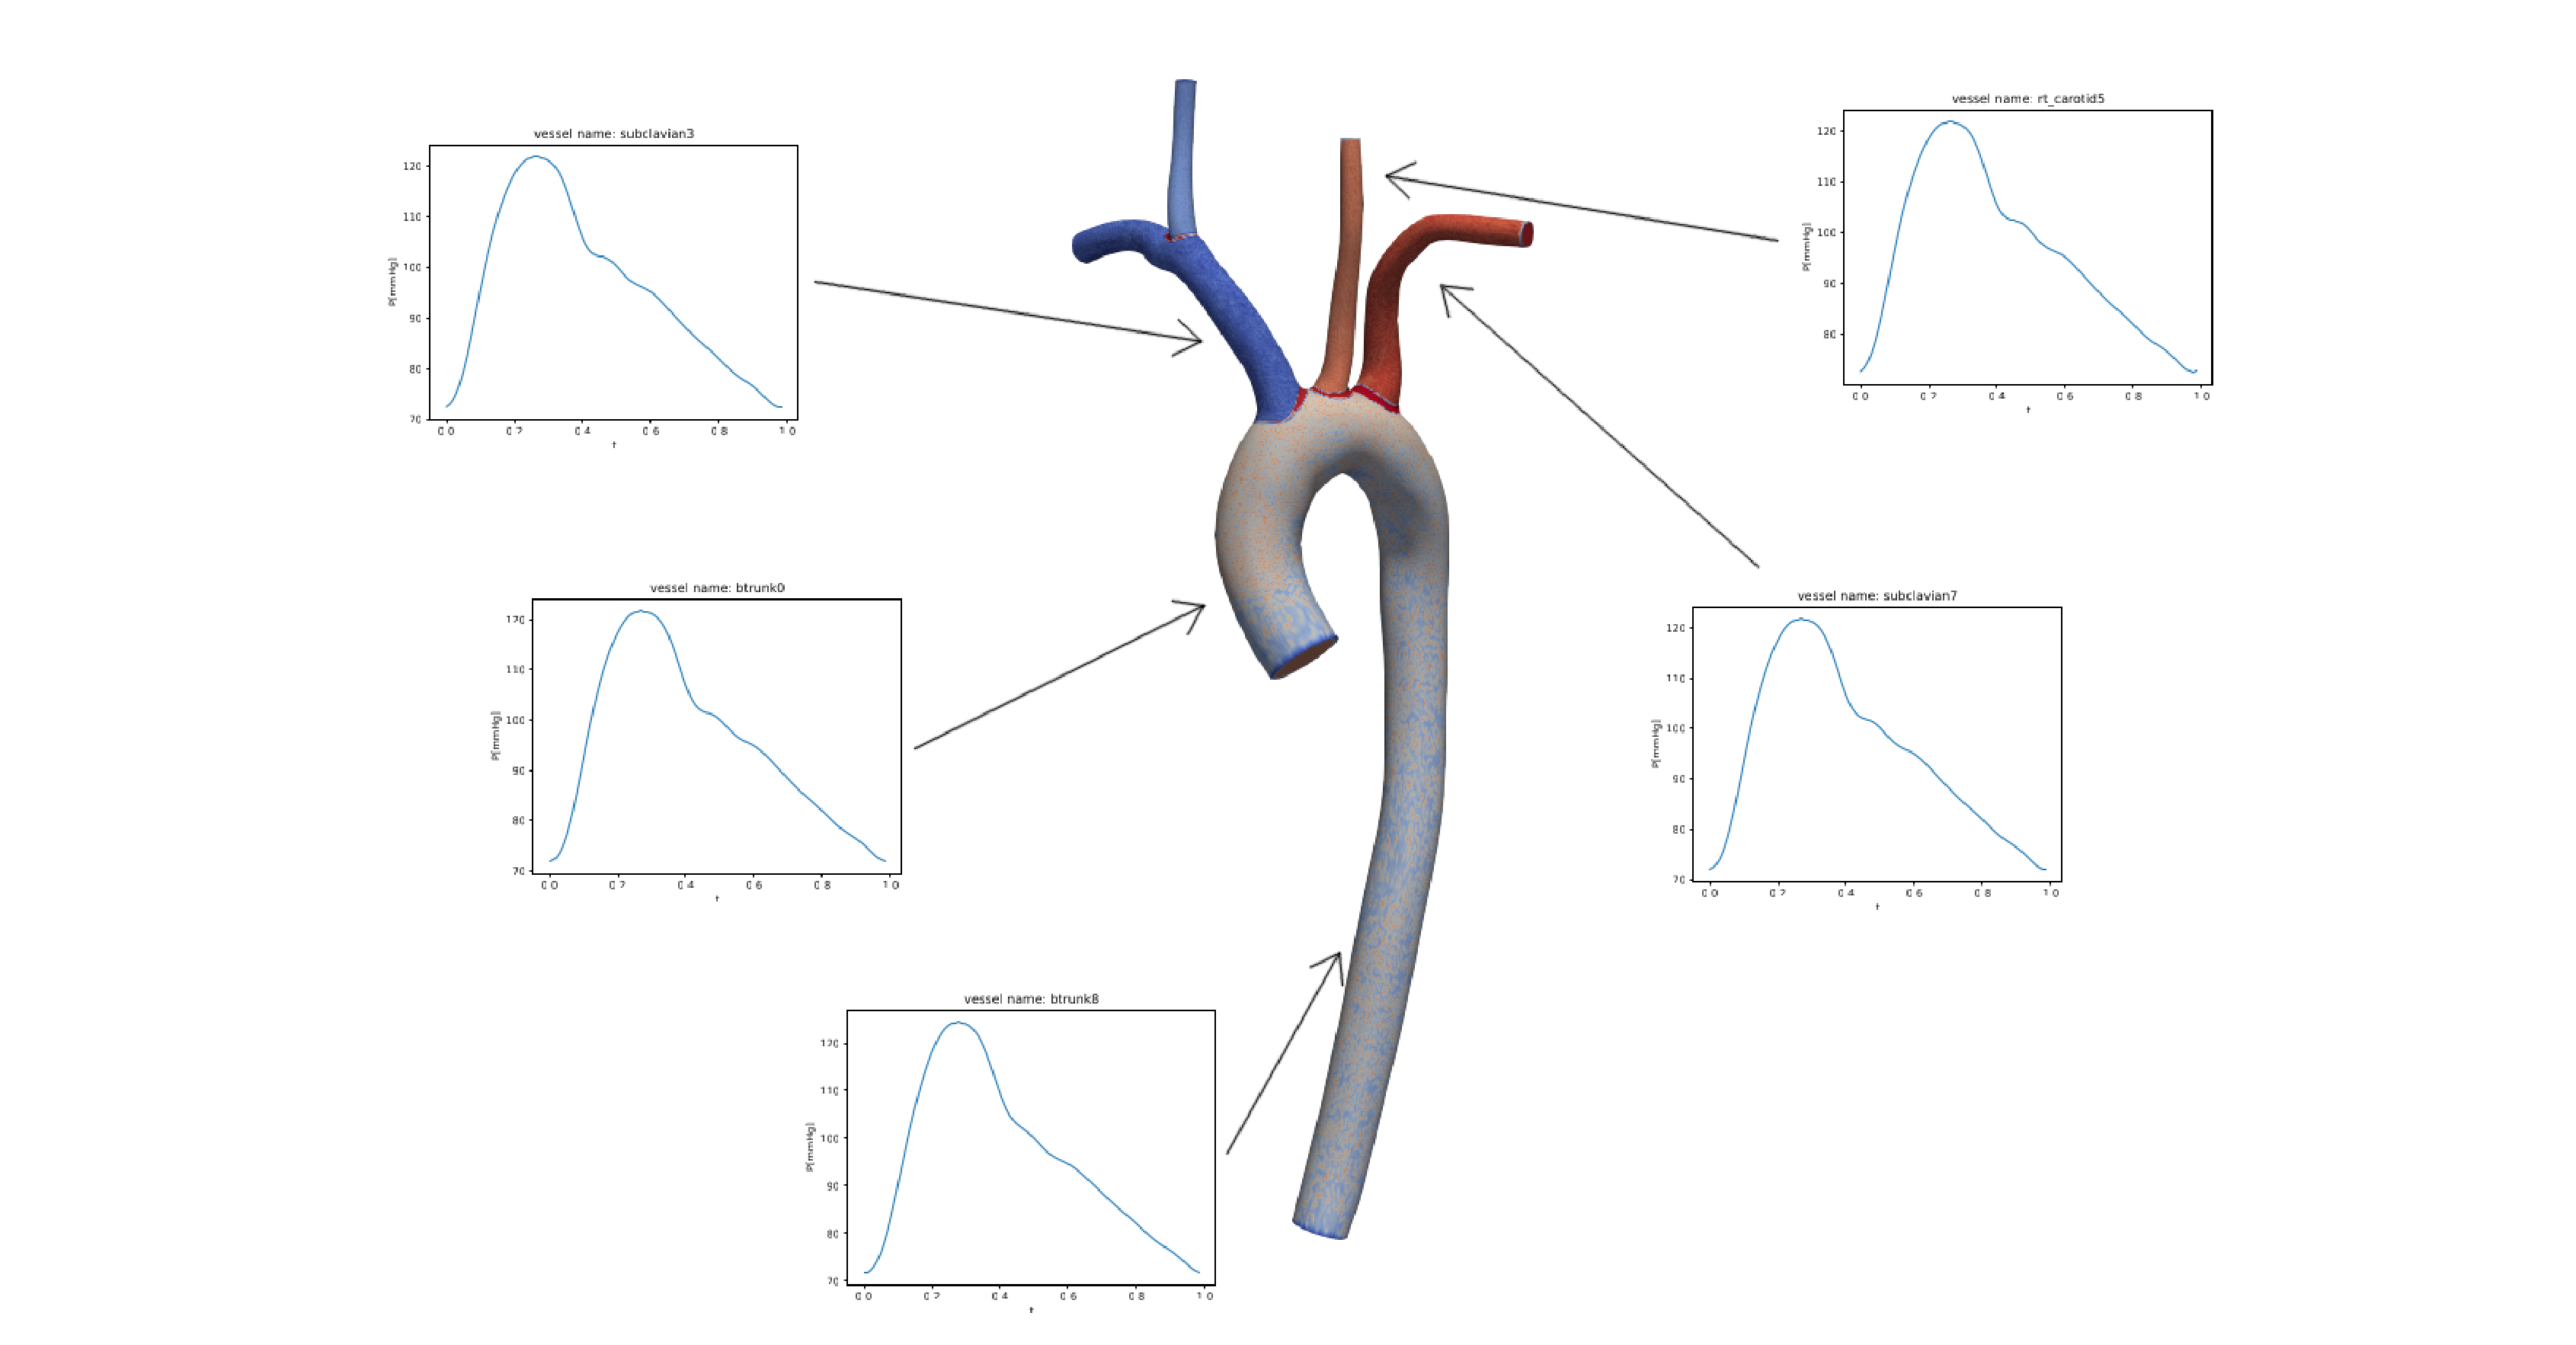
\includegraphics[width=0.8\columnwidth]{figures/0007_annotated.eps}
	\caption{The haemodynamics solver produces qualitatively accurate results for the 8 vessel aorta model.}
	\label{fig:aorta}
\end{figure}

The second \emph{vascularmodel.com} model, the abdominal model, consists of the following arteries: 
The right and left common, external, and internal iliac arteries, the right and left femoral arteries, as well as the right and left renal arteries, the celiac trunc and the superior mesentric artery.
The results from our simulation of the abdominal model can be seen in \autoref{fig:abdominal}.
\begin{figure} [!ht]
	\centering
	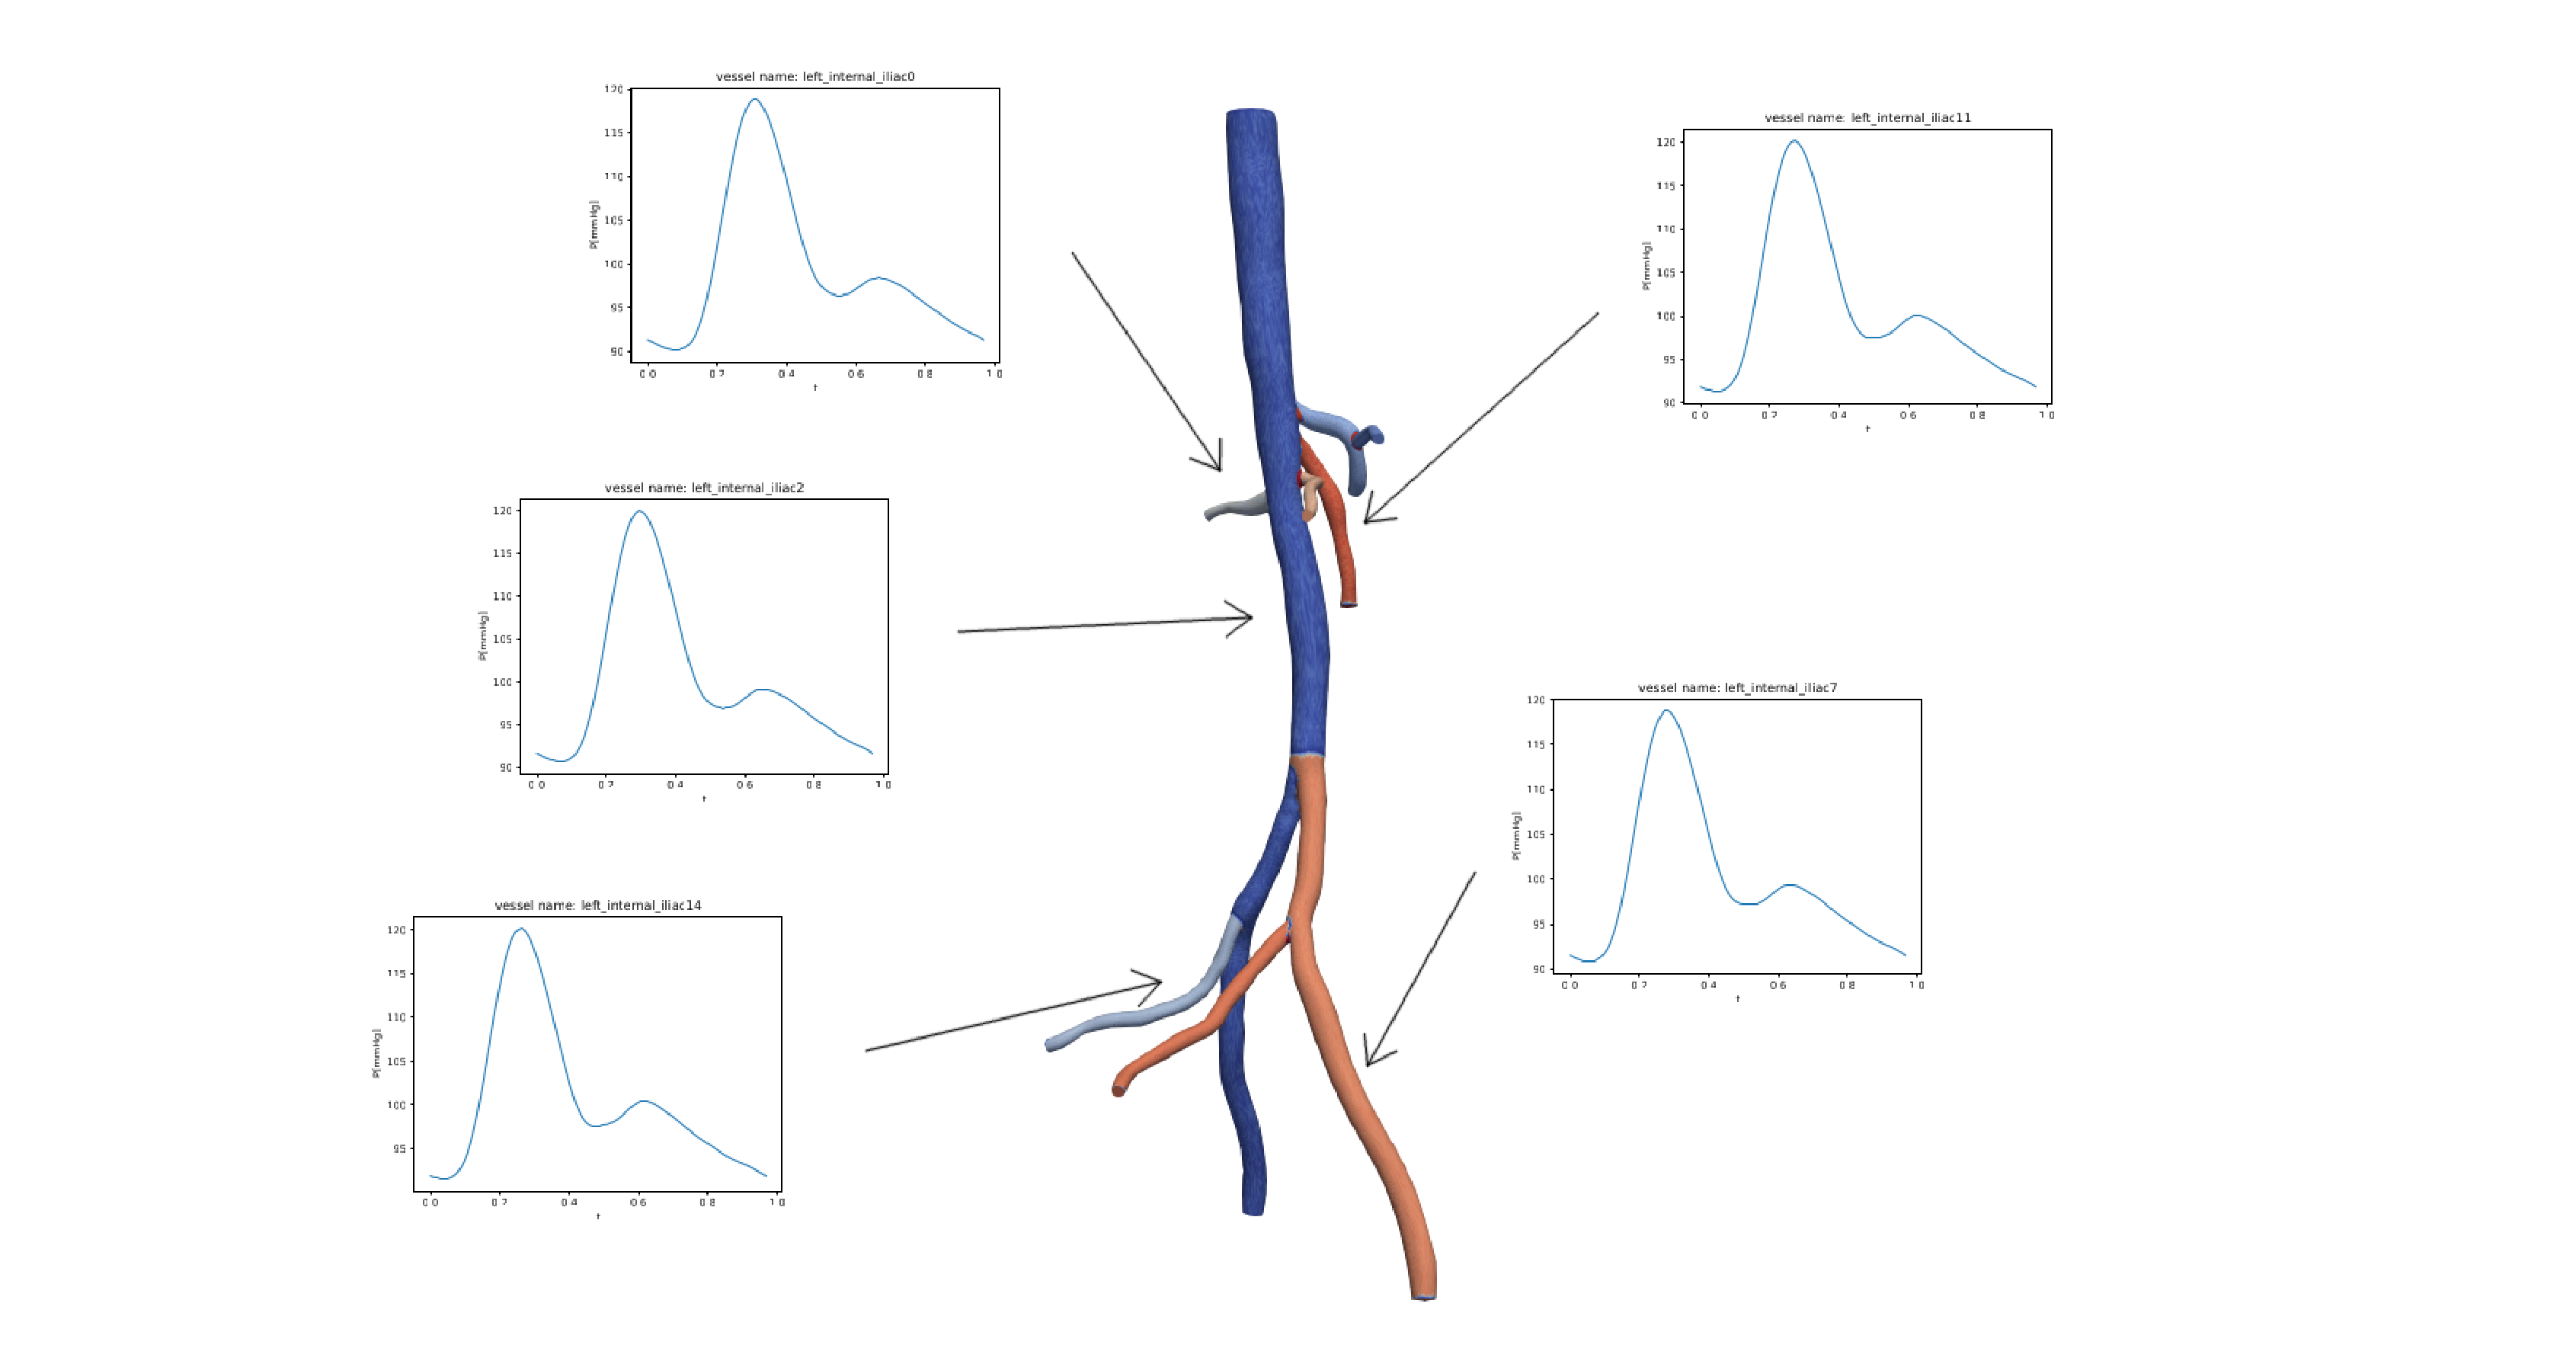
\includegraphics[width=0.8\columnwidth]{figures/0029_annotated.eps}
	\caption{The abdominal model consists of 12 models and is therefore slightly larger than the aorta model but can still be simulated accurately.}
	\label{fig:abdominal}
\end{figure}
Our final model from the \emph{vascularmodel.com} database models cerebral arteries.
It includes among others the right and left anterior inferior cerebellar arteries, vertebral arteries, and the second posterior cerebral artery.
The results from simulating the cerebral model are shown in \autoref{fig:cerebral}
\begin{figure} [!ht]
	\centering
	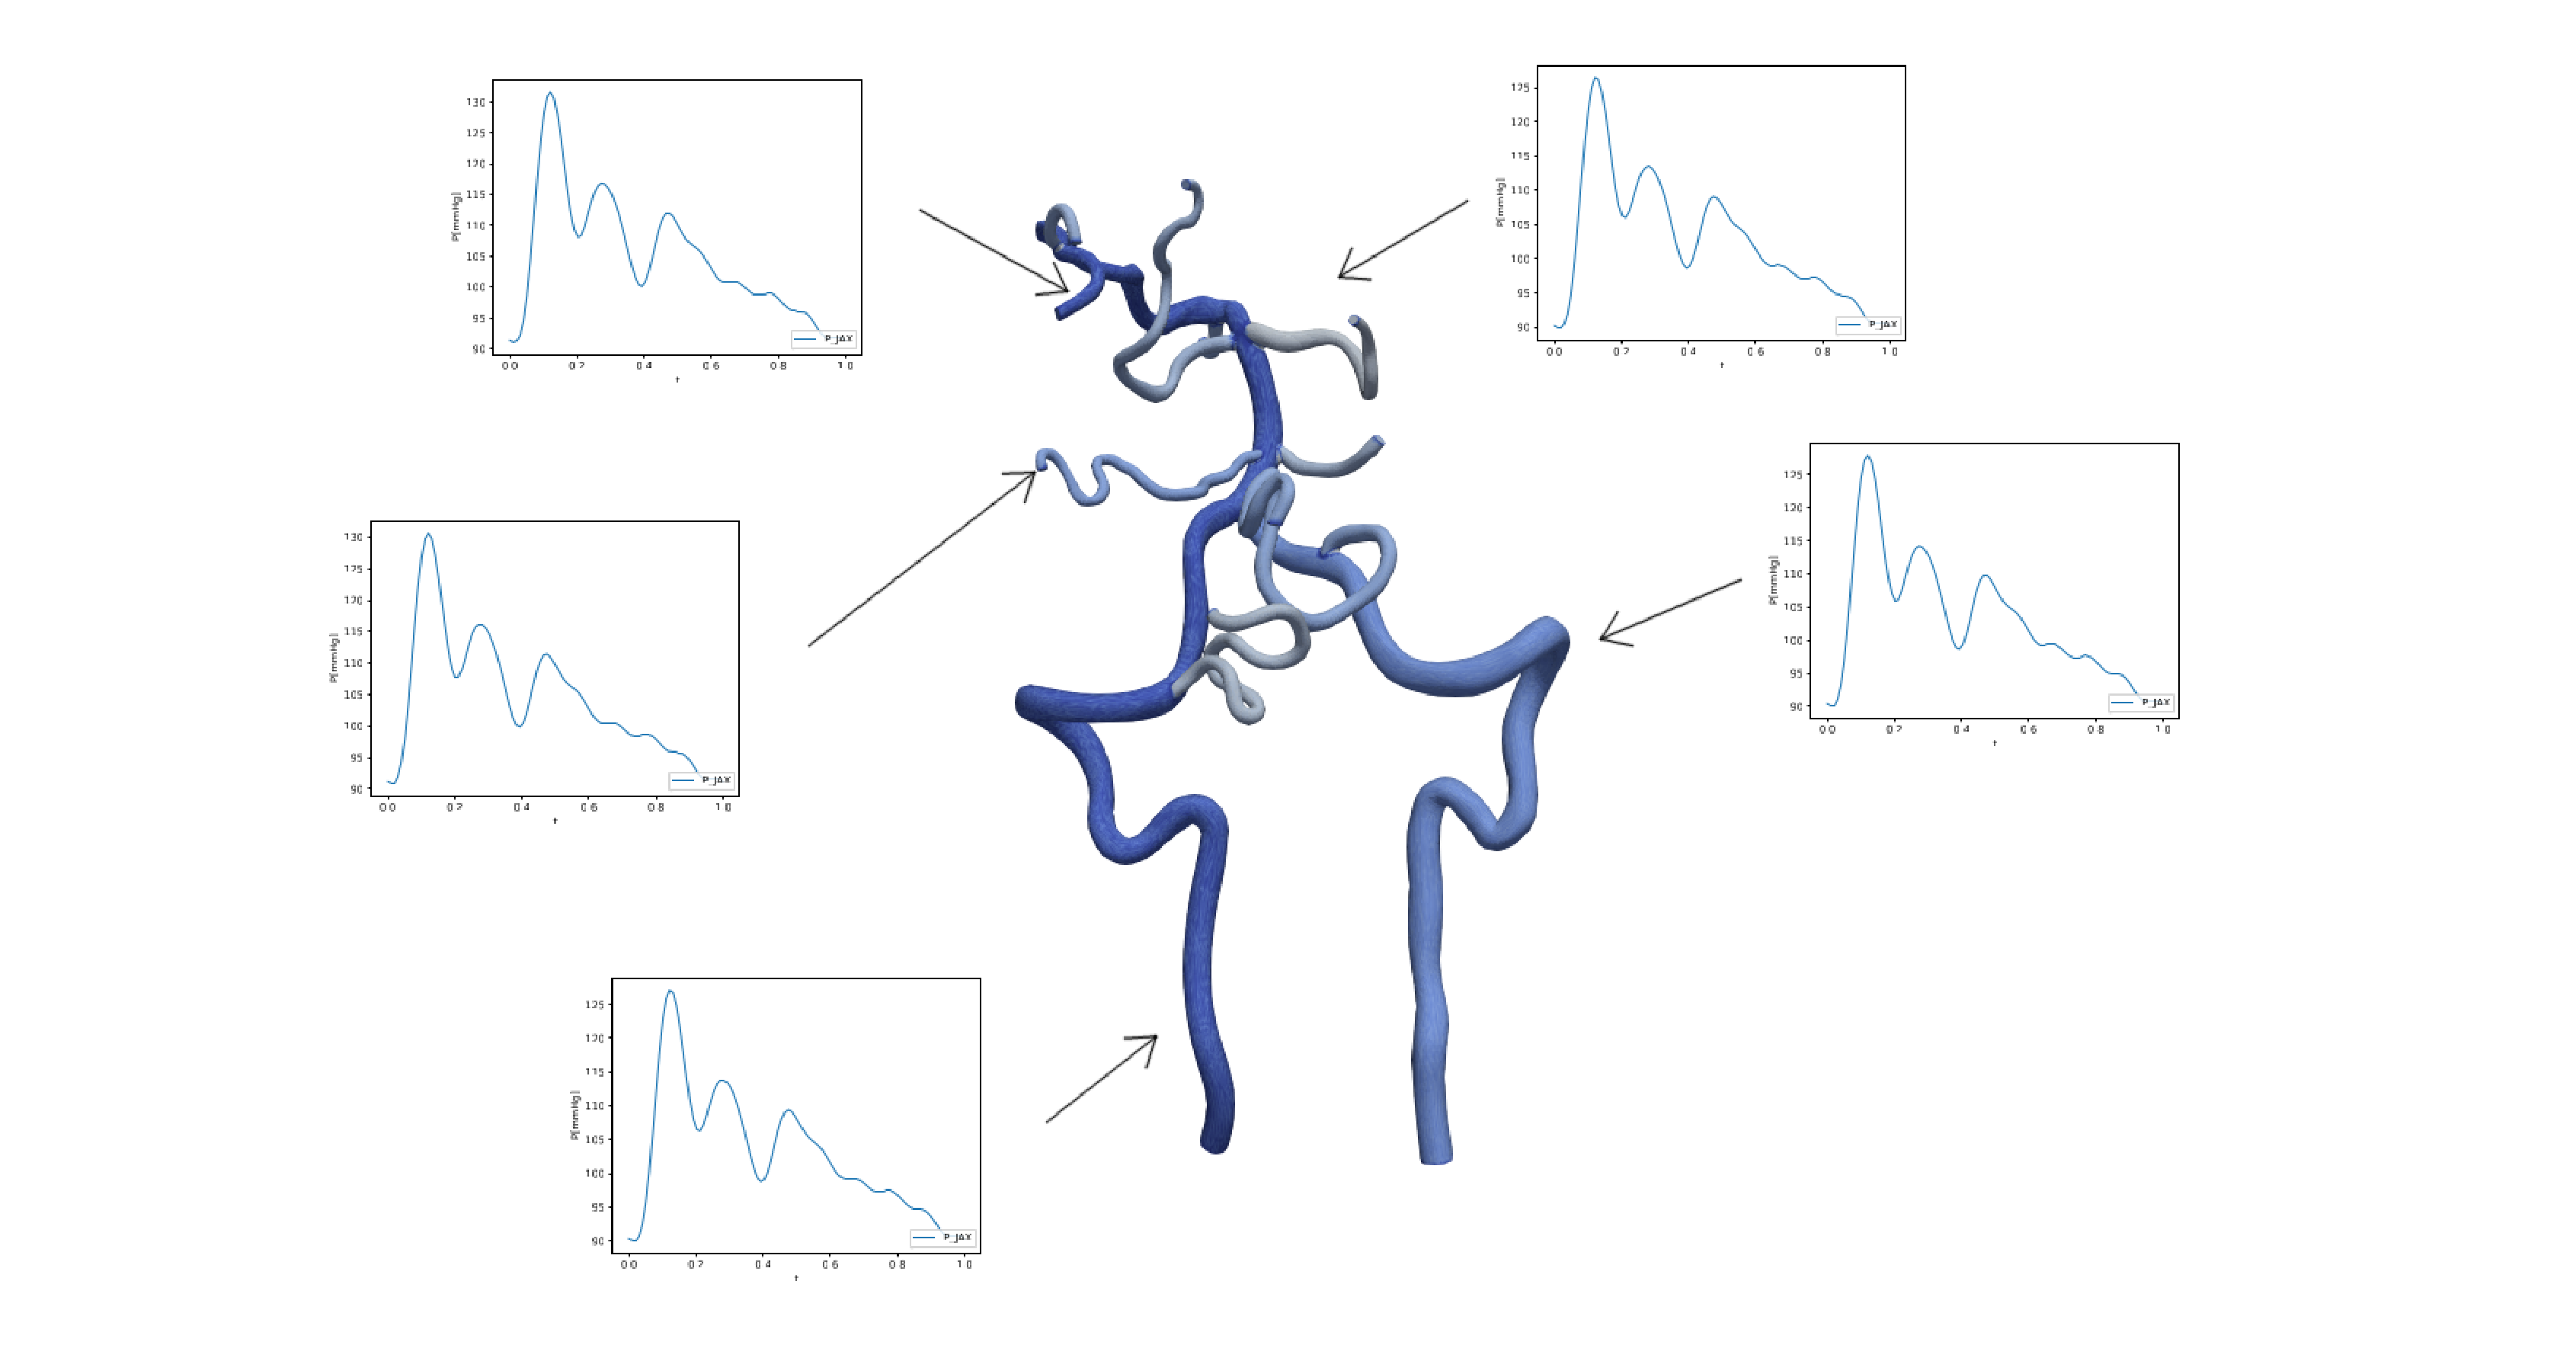
\includegraphics[width=0.8\columnwidth]{figures/0053_annotated.eps}
	\caption{The 10 vessel cerebral model provides reasonable results as well when simulated with our haemodynamics solver.}
	\label{fig:cerebral}
\end{figure}
Finally we turn to the "ADAN56" model.
With 56 vessels this is by far the biggest model presented here.
The input data here was inspired by \cite{murgo1980aortic}.
The results are visualized in \autoref{fig:adan56}.
\begin{figure} [!ht]
	\centering
	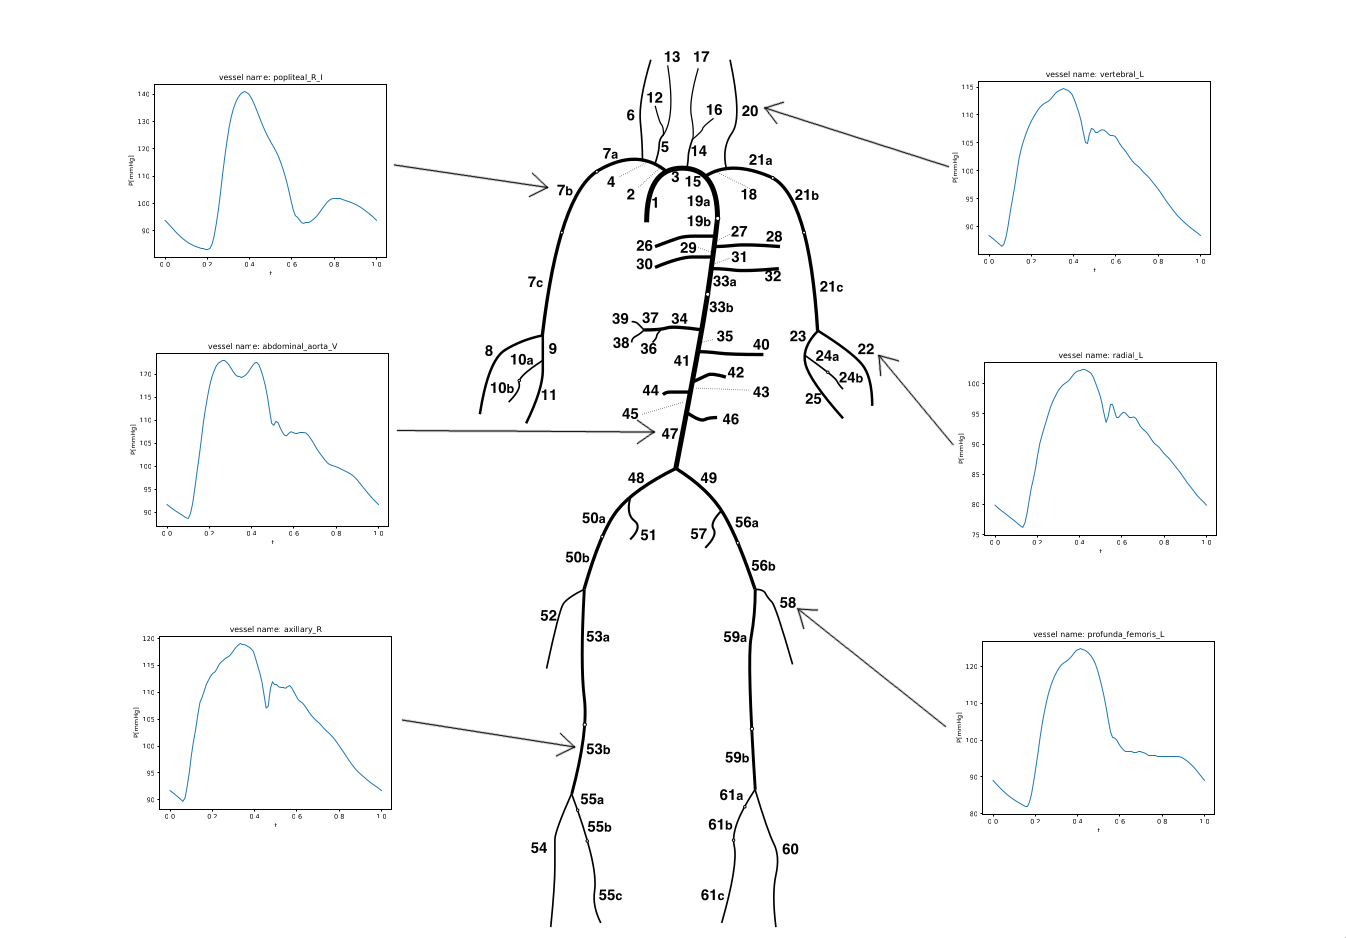
\includegraphics[width=0.8\columnwidth]{figures/adan56_annotated.png}
	\caption{The simulation results from the ADAN56 artery network show that larger systems can be simulated by our jax code as well.}
	\label{fig:adan56}
\end{figure}
A stark difference between the models from \emph{vascularmodel.com} and the ADAN56 model is how much variety there is in the different pulse waves generateed for different arteriees in the ADAN56 model as opposed to the ones generated for the other models.
This is most likely a result of the way the RCR parameters were set for these different models.
For the ADAN56 model the resistances and the compliance were carefully analized and calibrated in \cite{blanco2014anatomically,blanco2014blood} to provide a physiologically realistic result.
Due to the parameters not always being provided in the \emph{vascularmodel.com} models, here they were computed using a fairly simple approximation.
The total resistance of the system is computed as:
\begin{equation}
R_{tot} = \frac{P_{mean}}{Q_{car}}
\end{equation}
where the mean pressure $P_{mean}$ and the cardiac output $Q_{car}$ are set to the nominal values:
\begin{align}
	P_{mean} &= \frac{120 \text{mmHg}}{80 \frac{\text{ml}}{\text{s}}} \approx 2 \times 10^8 \frac{\text{kg}}{\text{m}^4\text{s}} \\
	Q_{car} &= 80 \frac{\text{ml}}{\text{s}} = 8 \times 10^{-5} \frac{\text{m}^3}{\text{s}}. \\
\end{align}
The total compliance is set to a reasonable value as well
\begin{align}
	C_{tot} &= 10^{-3} \frac{\text{cm}^5}{\text{dyne}} = 10^{-8} \frac{\text{m}^3}{\text{Pa}}.
\end{align}
The individual resistances and the compliances are then set using the rules for a parallel circuit.
Let $I$ be an index set containing all vessels with a windkessel outlet and $A_{o,i}, i \in I$ the reference cross-section at the outlet of the $i$-th vessel.
The resistance and the compliance at vessel $i$ are then computed by
\begin{align}
	\xi_i &= \frac{\sum_{j \in I} A_{0,j}}{A_{0,i}} \\
	R_{tot,i} &= \xi_i R_{tot} \\
	C_{tot,i} &= \frac{1}{\xi_i} R_{tot}. 
\end{align}
Finally the proximal and the distal resistance $R_{1,i}, R_{2,i}$ have to be set for each vessel $i$.
This is done by invoking an approximate ratio of about 1:10 between the two
\begin{align}
	R_{1,i} &= \frac{9}{100} R_{tot,i} \\
	R_{2,i} &= \frac{91}{100} R_{tot,i}.
\end{align}
This recipe was taken from the \emph{simvascular} documentation. \cite{simvascular}
Some of the resistances were manually fitted to better fit the specific model.
The different behaviour in the simulation for the meticoulously asigned parameters in the ADAN56 model as opposed to the approximated parameters assigned when simulating the \emph{vascularmodel.com} models demonstrates that there is no simple answer to calibrating the RCR prameters for the windkessel model.
Here the code written in this work can be seen as a step towards easier and more accurate procedures to determine such parameters.
Given data the differentiability of the code could be leveraged to perform parameter inference on precisely these parameters.
\section{Scaling} \label{sec:sc}
As mentioned in \autoref{sec:jax} on JAX there is a significant overhead to the compilation JAX performs in order to optimize.
This begs the question if the compilation dominates the total computation time and how the compilation time scales for growing numbers of vessel segments in a simulated network.
If the compilation time doesn't increase much even for larger models this would mean that for big enough systems the compilation overhead could pay off.
The compilation and total computation time have been plotted for simulations with different numbers of vessel segments in \autoref{fig:timing}
These timings were prduced on a Xeon E3-1505 v6 with 4 cores and 8 threads, a base frequency of 3.0GHz and a maximum turbo frequency of 4.0GHz, 8MB of cache, and 16GB of DDR4 memory clocked at 2400MT.
\begin{figure} [!ht]
	\centering
	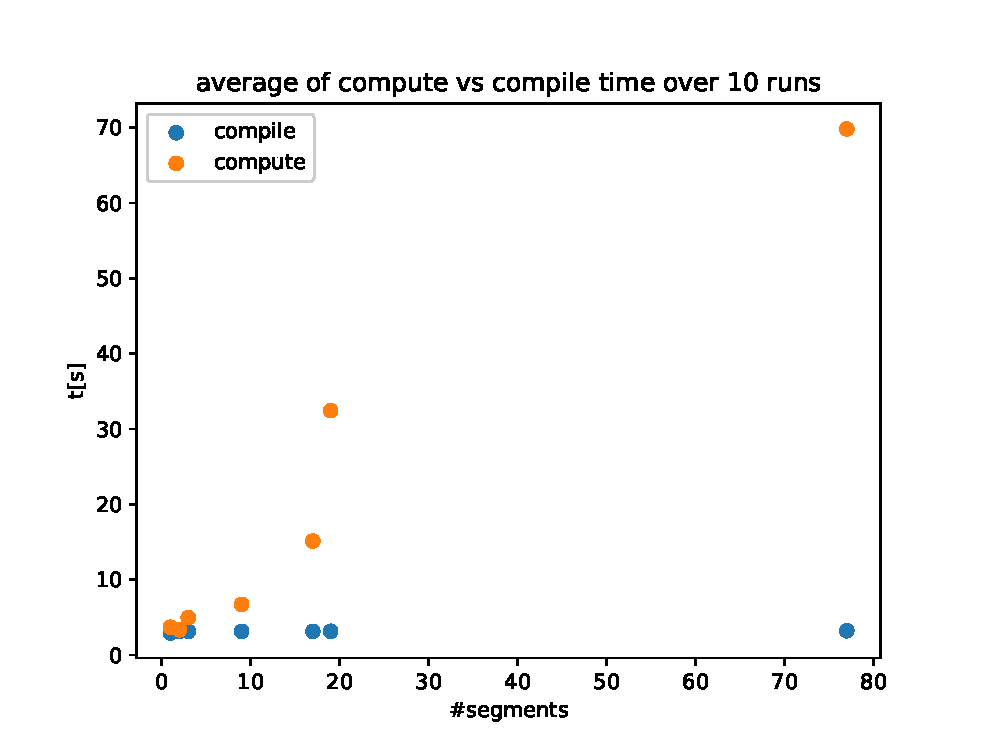
\includegraphics[width=0.8\columnwidth]{figures/timing.eps}
	\caption{The compile time doesn't grow significantly with increasing numbers of vessel segments due to builtin Python loops being avoided which would be costly to compile. Total compute times seem to scale linearly w.r.t. the number of vessel segments with the exception of the 20 vessel segment simulation.}
	\label{fig:timing}
\end{figure}
The compile time remains almost constant around 3s even as the number of vessel segments increases over two magnitudes of order.
This is due to the methods described in \autoref{ssec:al}.
Due to avoiding builtin python loops in favor of JAX loop constructions the compile time is kept more or less static since these kind of loops don't have to be unrolled during compilation.
Hence there is barely any additional effort involved with compiling for larger network simulations.
In general the compile time is only a fraction of the total compute time once a certain amount of vessels is considered in the simulation and becomes and it becomes insignificant with growing model sizes.
It can also be observed that total compute time shows linear scaling as a function of the number of vessel segments when considering the 20 vessel segment data point to be an outlier.
Convergence within a simulation is heavily dependent on the specific network that is being simulated.
Therefore it is reasonable to assume that there will be outliers when comparing the compute time between simulations with different underlying networks.


\section{Parameter Inference} \label{sec:pi}

\chapter{Conclusion/ Future Work}


% This displays the bibliography for all cited external documents. All references have to be defined in the file references.bib and can then be cited from within this document.
\bibliographystyle{IEEEtran}
\bibliography{references/references}

% This creates an appendix chapter, comment if not needed.
\appendix
\chapter{Code Documentation/ Manual} 


\end{document}

